\documentclass[11pt,a4paper]{article}

% --------------------------------------------------
% Packages
% --------------------------------------------------
\usepackage[margin=2.2cm]{geometry}
\usepackage{amsmath,amssymb,mathtools}
\usepackage{graphicx}
\usepackage{subcaption}
\usepackage{booktabs}
\usepackage{array}
\usepackage{multirow}
\usepackage{siunitx}
\usepackage{microtype}
\usepackage{enumitem}
\usepackage{xcolor}
\usepackage{hyperref}
\usepackage{fancyhdr}
\usepackage{float}
\usepackage{placeins}

\graphicspath{{figures/}}
\sisetup{scientific-notation=true,round-mode=figures,round-precision=4}

\hypersetup{
    colorlinks=true,
    linkcolor=blue!45!black,
    citecolor=blue!45!black,
    urlcolor=blue!45!black,
    pdftitle={Numerical Simulation of Single-Particle Drifts in Electromagnetic Fields},
    pdfauthor={Juan Pablo Solís Ruiz}
}

\pagestyle{fancy}
\fancyhf{}
\lhead{Single-Particle Drift Simulation}
\rhead{Fundamentals of Plasma Physics}
\cfoot{\thepage}
\setlength{\headheight}{14pt}

\newcommand{\vect}[1]{\boldsymbol{#1}}
\newcommand{\vE}{\vect{v}_{E}}
\newcommand{\vgradB}{\vect{v}_{\nabla B}}
\newcommand{\vc}{\vect{v}_{c}}
\newcommand{\vp}{\vect{v}_{p}}
\newcommand{\Ohm}{\Omega_c}
\newcommand{\rhL}{\rho_L}

\begin{document}

% --------------------------------------------------
% Title page
% --------------------------------------------------
\begin{titlepage}
    \centering
    \vspace*{2.0cm}

    {\Large University of Science and Technology of China (USTC)\par}
    \vspace{1.1cm}

    {\huge\bfseries Numerical Simulation of Single-Particle Drifts\par}
    \vspace{0.25cm}
    {\huge\bfseries in Prescribed Electromagnetic Fields\par}

    \vspace{1.4cm}
    {\Large Fundamentals of Plasma Physics\par}

    \vfill

    \begin{tabular}{rl}
        \textbf{Student:} & Juan Pablo Solís Ruiz \\
        \textbf{Program:} & M.Sc. Physics - Plasma Physics \\
        \textbf{Method:} & C++17 full-orbit integration + Python validation \\
	\textbf{Repository:} & \url{https://github.com/h4xter1612/charged_particle_sim} \\
        \textbf{Date:} & October 2026
    \end{tabular}

    \vfill


\end{titlepage}

\section*{Abstract}
A three-dimensional full-orbit simulator was implemented in C++17 to study single-particle drift motion in prescribed electromagnetic fields. The normalized Lorentz equations are integrated with a fourth-order Runge-Kutta method, while independent Python scripts are used for analytical comparison, guiding-center diagnostics, conservation checks, and visualization. The five required cases--$E\times B$, grad-$B$, curvature, spatially nonuniform electric field, and polarization drift--are reproduced directly from the full Lorentz dynamics. A uniform-$B$ benchmark verifies the integrator before nonuniform fields are introduced. Exact-solvable cases agree with analytical full-orbit solutions at approximately $10^{-9}$--$10^{-11}$, while the nonuniform cases reproduce the expected guiding-center and finite-Larmor-radius corrections.

\tableofcontents
\newpage

% --------------------------------------------------
\section{Objective and Scope}
% --------------------------------------------------

The objective of this project is to simulate the full orbit of a charged particle in prescribed electromagnetic fields and to recover, from the Lorentz dynamics, the drift motions discussed in class. The five required cases are
\begin{enumerate}[label=\arabic*.]
    \item uniform crossed-field $\vect{E}\times\vect{B}$ drift,
    \item magnetic-gradient ($\nabla B$) drift,
    \item curvature drift,
    \item drift in a spatially nonuniform electric field, and
    \item polarization drift in a time-dependent electric field.
\end{enumerate}

A sixth case, motion in a uniform magnetic field, is used as a numerical benchmark before introducing any drift-producing nonuniformity. The C++ program integrates the complete Lorentz-force equations; no drift velocity is inserted directly into the equations of motion. Python scripts are then used to analyze the generated CSV trajectories, compare with analytical or guiding-center theory, evaluate conservation laws, and generate the figures in this report.

% --------------------------------------------------
\section{Physical Model and Normalization}
% --------------------------------------------------

\subsection{Lorentz equations}

The dimensional equations for a particle of charge $q$ and mass $m$ are
\begin{align}
    \frac{d\vect{r}}{dt} &= \vect{v}, \\
    m\frac{d\vect{v}}{dt} &= q\left[\vect{E}(\vect{r},t)+\vect{v}\times\vect{B}(\vect{r},t)\right].
    \label{eq:lorentz_dimensional}
\end{align}
The magnetic part of the Lorentz force is perpendicular to the instantaneous velocity and therefore performs no work. When $\vect{E}=0$, the kinetic energy should remain constant; when an electrostatic or time-dependent electric field is present, the appropriate energy or work relation is used instead.

\subsection{Dimensionless variables}

The simulations are performed in normalized units. Let $B_{\rm ref}$, $v_{\rm ref}$, $m_{\rm ref}$, and $|q_{\rm ref}|$ be reference quantities and define
\begin{equation}
    \Omega_{\rm ref}=\frac{|q_{\rm ref}|B_{\rm ref}}{m_{\rm ref}},
    \qquad
    t_{\rm ref}=\Omega_{\rm ref}^{-1},
    \qquad
    \rho_{\rm ref}=\frac{v_{\rm ref}}{\Omega_{\rm ref}},
    \qquad
    E_{\rm ref}=v_{\rm ref}B_{\rm ref}.
\end{equation}
The dimensionless variables are
\begin{equation}
    \vect{r}=\rho_{\rm ref}\,\tilde{\vect{r}},\quad
    t=t_{\rm ref}\tilde t,\quad
    \vect{v}=v_{\rm ref}\tilde{\vect{v}},\quad
    \vect{B}=B_{\rm ref}\tilde{\vect{B}},\quad
    \vect{E}=E_{\rm ref}\tilde{\vect{E}}.
\end{equation}
Writing $q=|q_{\rm ref}|\tilde q$ and $m=m_{\rm ref}\tilde m$ gives
\begin{align}
    \frac{d\tilde{\vect{r}}}{d\tilde t} &= \tilde{\vect{v}},\\
    \frac{d\tilde{\vect{v}}}{d\tilde t}
    &=\frac{\tilde q}{\tilde m}
    \left(\tilde{\vect{E}}+\tilde{\vect{v}}\times\tilde{\vect{B}}\right).
    \label{eq:lorentz_normalized}
\end{align}
The tildes are omitted in the code and throughout the rest of the report. For the benchmarks here, the reference species is used, so $m=1$ and $q=+1$. This normalization makes the cyclotron time and Larmor-radius scales explicit while preserving the $q/m$ dependence needed for the drift physics.

For a locally uniform field, the characteristic quantities are
\begin{equation}
    \Ohm=\frac{|q|B}{m},
    \qquad
    T_c=\frac{2\pi}{\Ohm},
    \qquad
    \rhL=\frac{v_\perp}{\Ohm}.
\end{equation}

% --------------------------------------------------
\section{Numerical Method and Code Organization}
% --------------------------------------------------

The coupled first-order system in Eq.~\eqref{eq:lorentz_normalized} is advanced with a classical fourth-order Runge-Kutta (RK4) scheme using $\Delta t=0.01$ in every benchmark. At each time step, the RK4 routine evaluates both $d\vect{r}/dt=\vect{v}$ and the Lorentz acceleration at four intermediate states. The field functions are evaluated at the corresponding intermediate position and time, which is essential for the nonuniform and time-dependent cases.

The project is intentionally separated into small components:
\begin{table}[H]
    \centering
    \caption{Main source files and responsibilities.}
    \begin{tabular}{p{0.27\textwidth}p{0.64\textwidth}}
        \toprule
        \textbf{File} & \textbf{Role} \\
        \midrule
        \texttt{Vec3.hpp} & Three-dimensional vector arithmetic, dot product, norm, and cross product. \\
        \texttt{Particle.hpp} & Particle position, velocity, normalized mass and charge, and kinetic energy. \\
        \texttt{Fields.hpp/.cpp} & Electromagnetic field models for the six benchmark cases. \\
        \texttt{Integrator.hpp/.cpp} & Lorentz acceleration and RK4 full-orbit time integration. \\
        \texttt{main.cpp} & Initial conditions, benchmark parameters, basic validation, and CSV output. \\
        \texttt{analysis/*.py} & Independent analytical checks, guiding-center diagnostics, fits, conservation tests, and visualization. \\
        \bottomrule
    \end{tabular}
\end{table}

The simulator writes
\begin{center}
\texttt{t, x, y, z, vx, vy, vz, kinetic\_energy}
\end{center}
to a CSV file. The Python analysis is deliberately kept separate from the C++ integrator so that analytical formulas are not used to generate the simulated trajectory itself.

\subsection{Benchmark parameters}

\begin{table}[H]
    \centering
    \small
    \caption{Normalized parameters used in the simulations.}
    \resizebox{\textwidth}{!}{%
    \begin{tabular}{llllll}
        \toprule
        \textbf{Case} & $\vect{r}(0)$ & $\vect{v}(0)$ & \textbf{Field parameters} & $\Delta t$ & $t_{\rm final}$ \\
        \midrule
        Uniform $B$ & $(0,0,0)$ & $(1,0,0.2)$ & $B_0=1$ & 0.01 & 20 \\
        $E\times B$ & $(0,0,0)$ & $(1,0,0.2)$ & $B_0=1,\ E_0=0.1$ & 0.01 & 20 \\
        Grad-$B$ & $(0,0,0)$ & $(1,0,0.2)$ & $B_0=1,\ g=0.05$ & 0.01 & 100 \\
        Curvature & $(10,0,0)$ & $(0.2,1,0)$ & $B_0=1$ & 0.01 & 100 \\
        Nonuniform $E$ & $(0,0,0)$ & $(1,0,0.2)$ & $B_0=1,\ E_0=0.02,\ k=0.4$ & 0.01 & 60 \\
        Polarization & $(0,0,0)$ & $(0,-0.2,0.2)$ & $B_0=1,\ E_0=0.2,\omega_E=0.05$ & 0.01 & 250 \\
        \bottomrule
    \end{tabular}}
\end{table}

% --------------------------------------------------
\section{Uniform-Magnetic-Field Validation}
% --------------------------------------------------

Before studying drift motion, the integrator is tested with
\begin{equation}
    \vect{B}=\hat{\vect{z}},\qquad \vect{E}=0,
\end{equation}
and $\vect{v}(0)=(1,0,0.2)$. Since $q=m=B_0=1$, $\Ohm=1$, $\rhL=1$, and the exact solution is
\begin{align}
    v_x &= \cos t, & v_y &= -\sin t, & v_z &= 0.2,\\
    x &= \sin t, & y &= \cos t-1, & z &= 0.2t.
\end{align}
The orbit is therefore circular in the perpendicular plane and helical in three dimensions. The maximum absolute errors are approximately $1.6\times10^{-9}$ in $x$ and $y$, while the maximum relative kinetic-energy error is $2.69\times10^{-11}$.

\begin{figure}[H]
    \centering
    \begin{subfigure}[t]{0.54\textwidth}
        \centering
        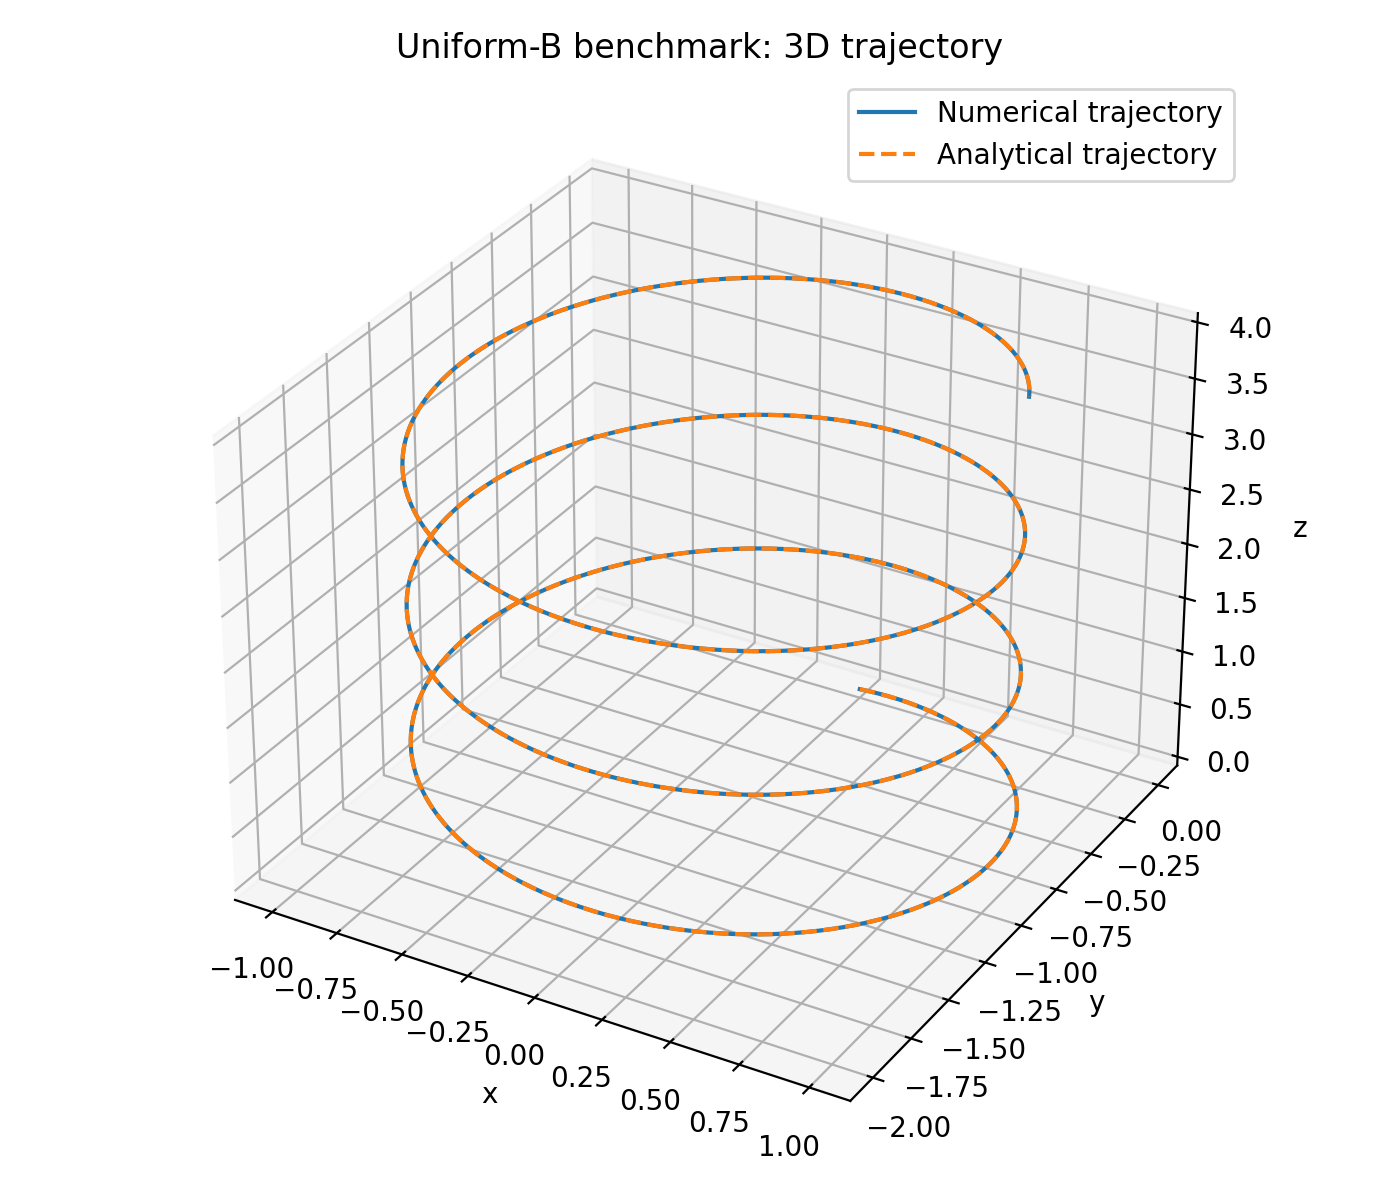
\includegraphics[width=\linewidth]{uniform_B_3d_trajectory.png}
        \caption{Three-dimensional helical orbit.}
    \end{subfigure}\hfill
    \begin{subfigure}[t]{0.44\textwidth}
        \centering
        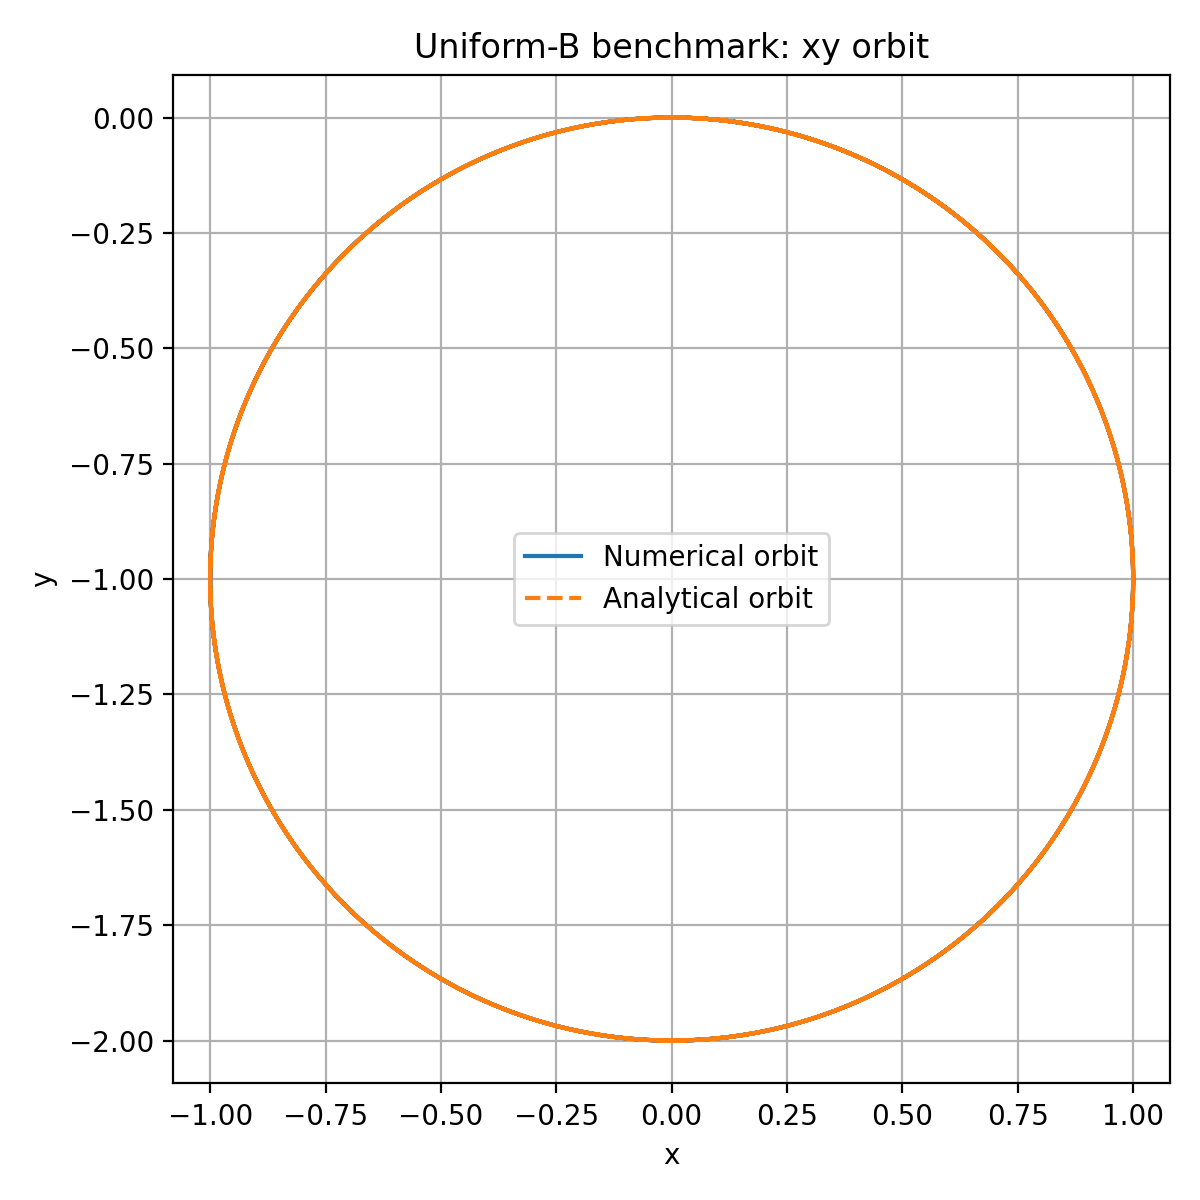
\includegraphics[width=\linewidth]{uniform_B_xy_orbit.png}
        \caption{Perpendicular circular orbit.}
    \end{subfigure}
    \caption{Uniform-$B$ benchmark. Numerical and analytical trajectories overlap at the plotted scale.}
    \label{fig:uniformB}
\end{figure}

This benchmark verifies the vector cross product, Lorentz acceleration, RK4 stage construction, and CSV output before additional field structure is introduced.

% --------------------------------------------------
\section{Required Drift Cases}
% --------------------------------------------------

\subsection{E x B drift}

For uniform crossed fields
\begin{equation}
    \vect{E}=E_0\hat{\vect{x}},\qquad
    \vect{B}=B_0\hat{\vect{z}},
\end{equation}
the guiding-center drift is
\begin{equation}
    \boxed{\vE=\frac{\vect{E}\times\vect{B}}{B^2}}
    =-\frac{E_0}{B_0}\hat{\vect{y}}.
    \label{eq:exb}
\end{equation}
This drift is independent of particle mass and charge. With $E_0=0.1$ and $B_0=1$, the expected drift is $v_{E,y}=-0.1$. A linear fit to the reconstructed numerical guiding center gives $-0.10000000$, with a relative difference of approximately $1.1\times10^{-13}$. The complete numerical particle orbit also agrees with the exact full-orbit solution to about $10^{-9}$ in position.

\begin{figure}[H]
    \centering
    \begin{subfigure}[t]{0.39\textwidth}
        \centering
        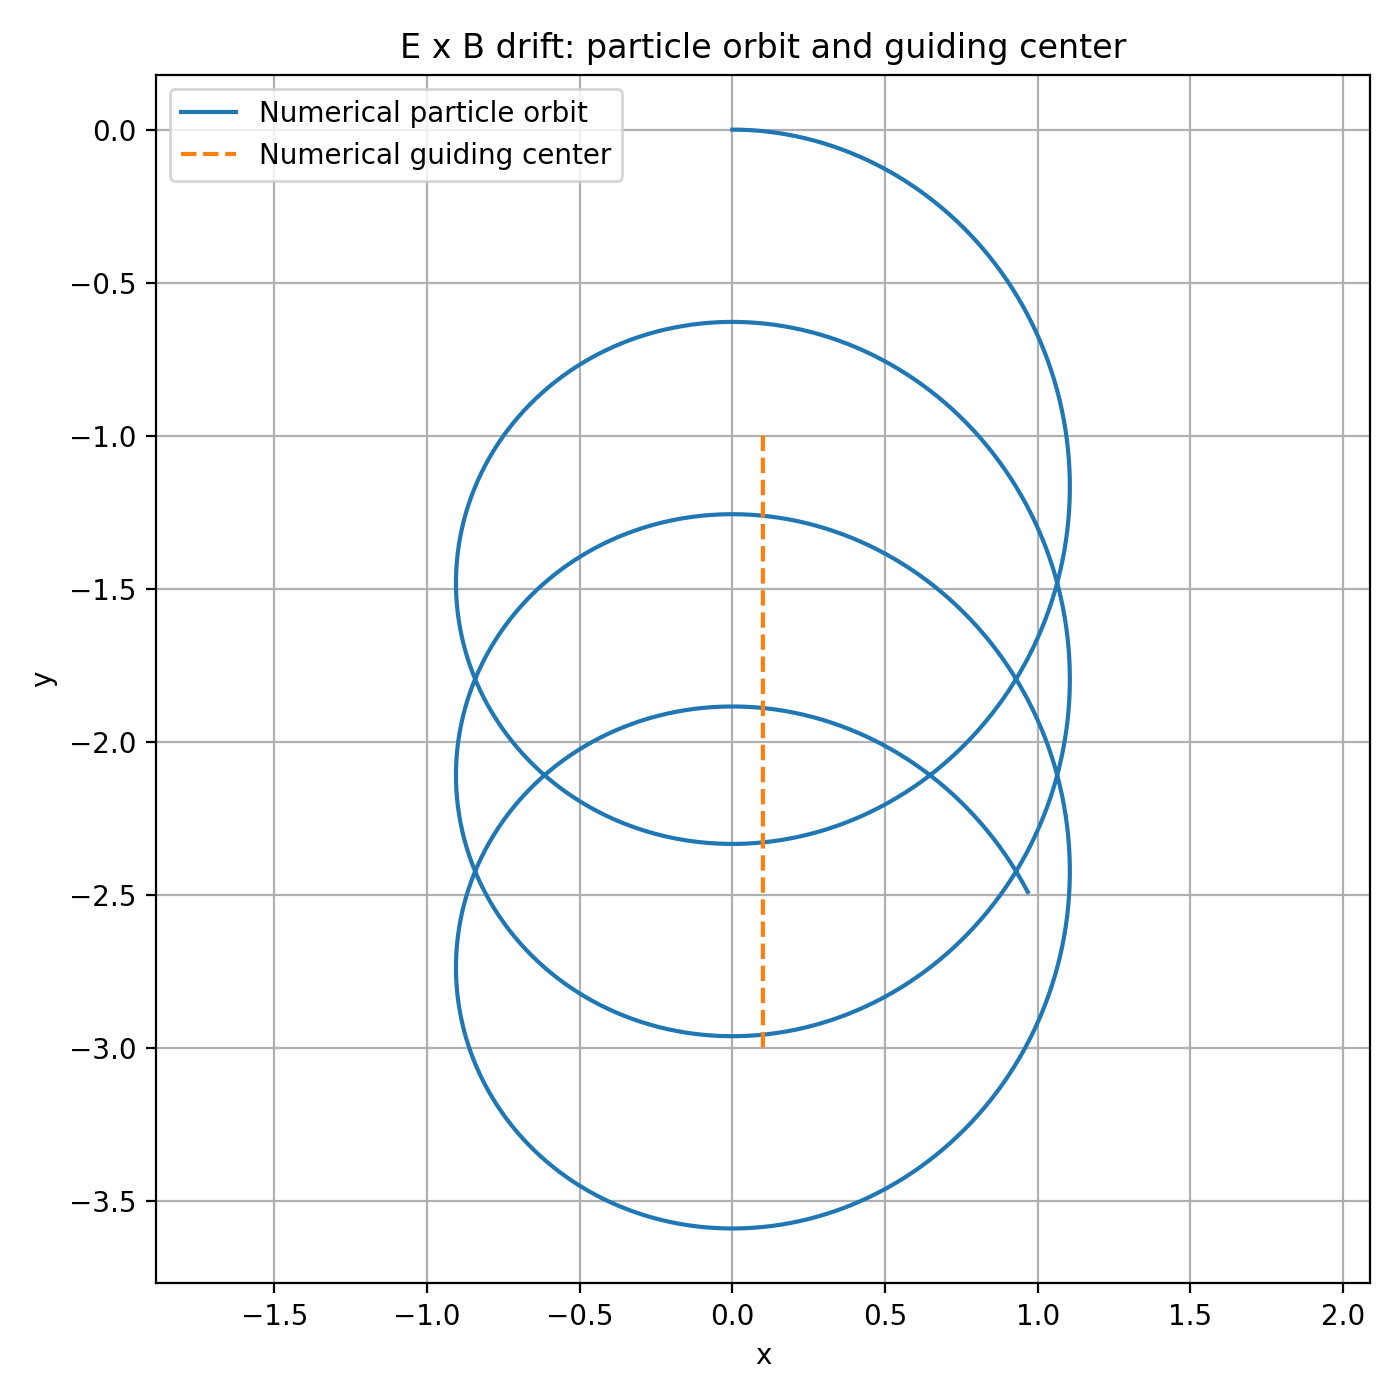
\includegraphics[width=\linewidth]{exb_xy_orbit.png}
        \caption{Gyromotion superimposed on the transverse drift.}
    \end{subfigure}\hfill
    \begin{subfigure}[t]{0.59\textwidth}
        \centering
        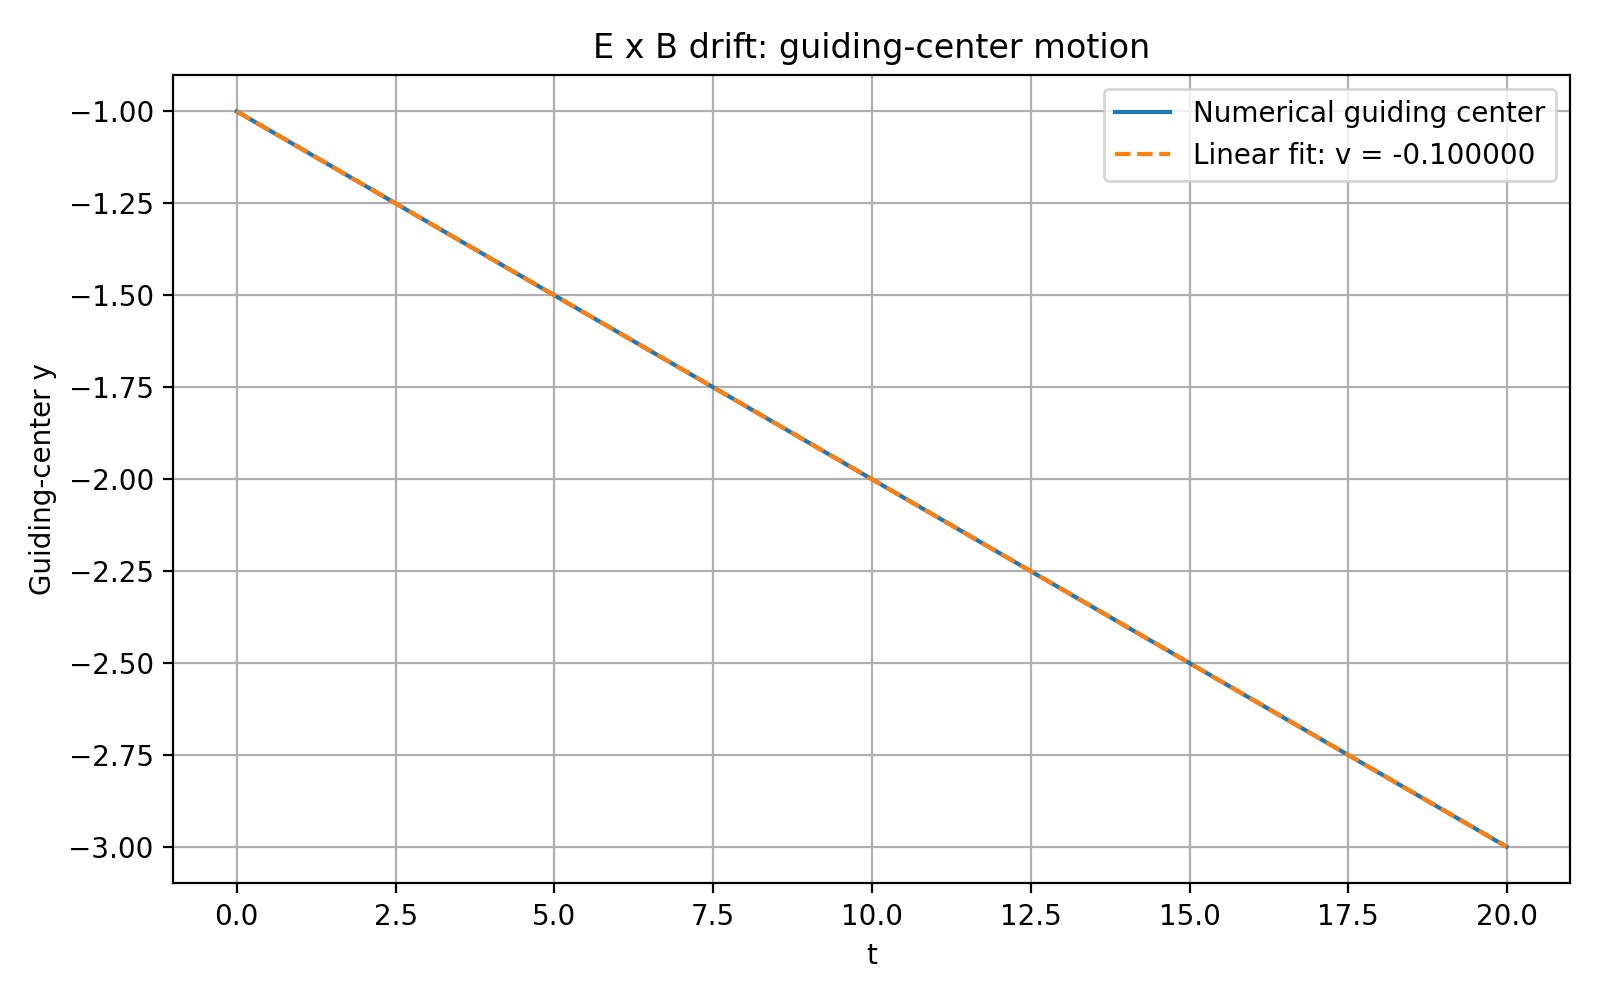
\includegraphics[width=\linewidth]{exb_guiding_center.png}
        \caption{Guiding-center displacement and linear fit.}
    \end{subfigure}
    \caption{$\vect{E}\times\vect{B}$ drift. The full orbit produces the theoretical guiding-center velocity without inserting the drift formula into the C++ equations.}
    \label{fig:exb}
\end{figure}

\subsection{Magnetic-gradient drift}

To isolate a magnetic-field gradient, the field is chosen as
\begin{equation}
    \vect{B}(x)=B_0(1+gx)\hat{\vect{z}},\qquad \vect{E}=0,
    \label{eq:gradbfield}
\end{equation}
with $g=0.05$. This field satisfies $\nabla\cdot\vect{B}=0$ because $B_z$ depends on $x$ but not on $z$.

The magnetic moment and first-order grad-$B$ drift are
\begin{equation}
    \mu=\frac{m v_\perp^2}{2B},
    \qquad
    \boxed{\vgradB=\frac{\mu}{qB^2}\vect{B}\times\nabla B}.
    \label{eq:gradb}
\end{equation}
Initially, $\rhL=1$ and the magnetic scale length is
\begin{equation}
    L_B=\frac{B}{|\nabla B|}=20,
    \qquad
    \epsilon_B=\frac{\rhL}{L_B}=0.05,
\end{equation}
so guiding-center theory should be accurate to low order. The first-order prediction is $v_{\nabla B,y}=0.025000$, whereas the numerical value is $0.02506606$, a relative difference of $0.264\%$.

\begin{figure}[H]
    \centering
    \begin{subfigure}[t]{0.42\textwidth}
        \centering
        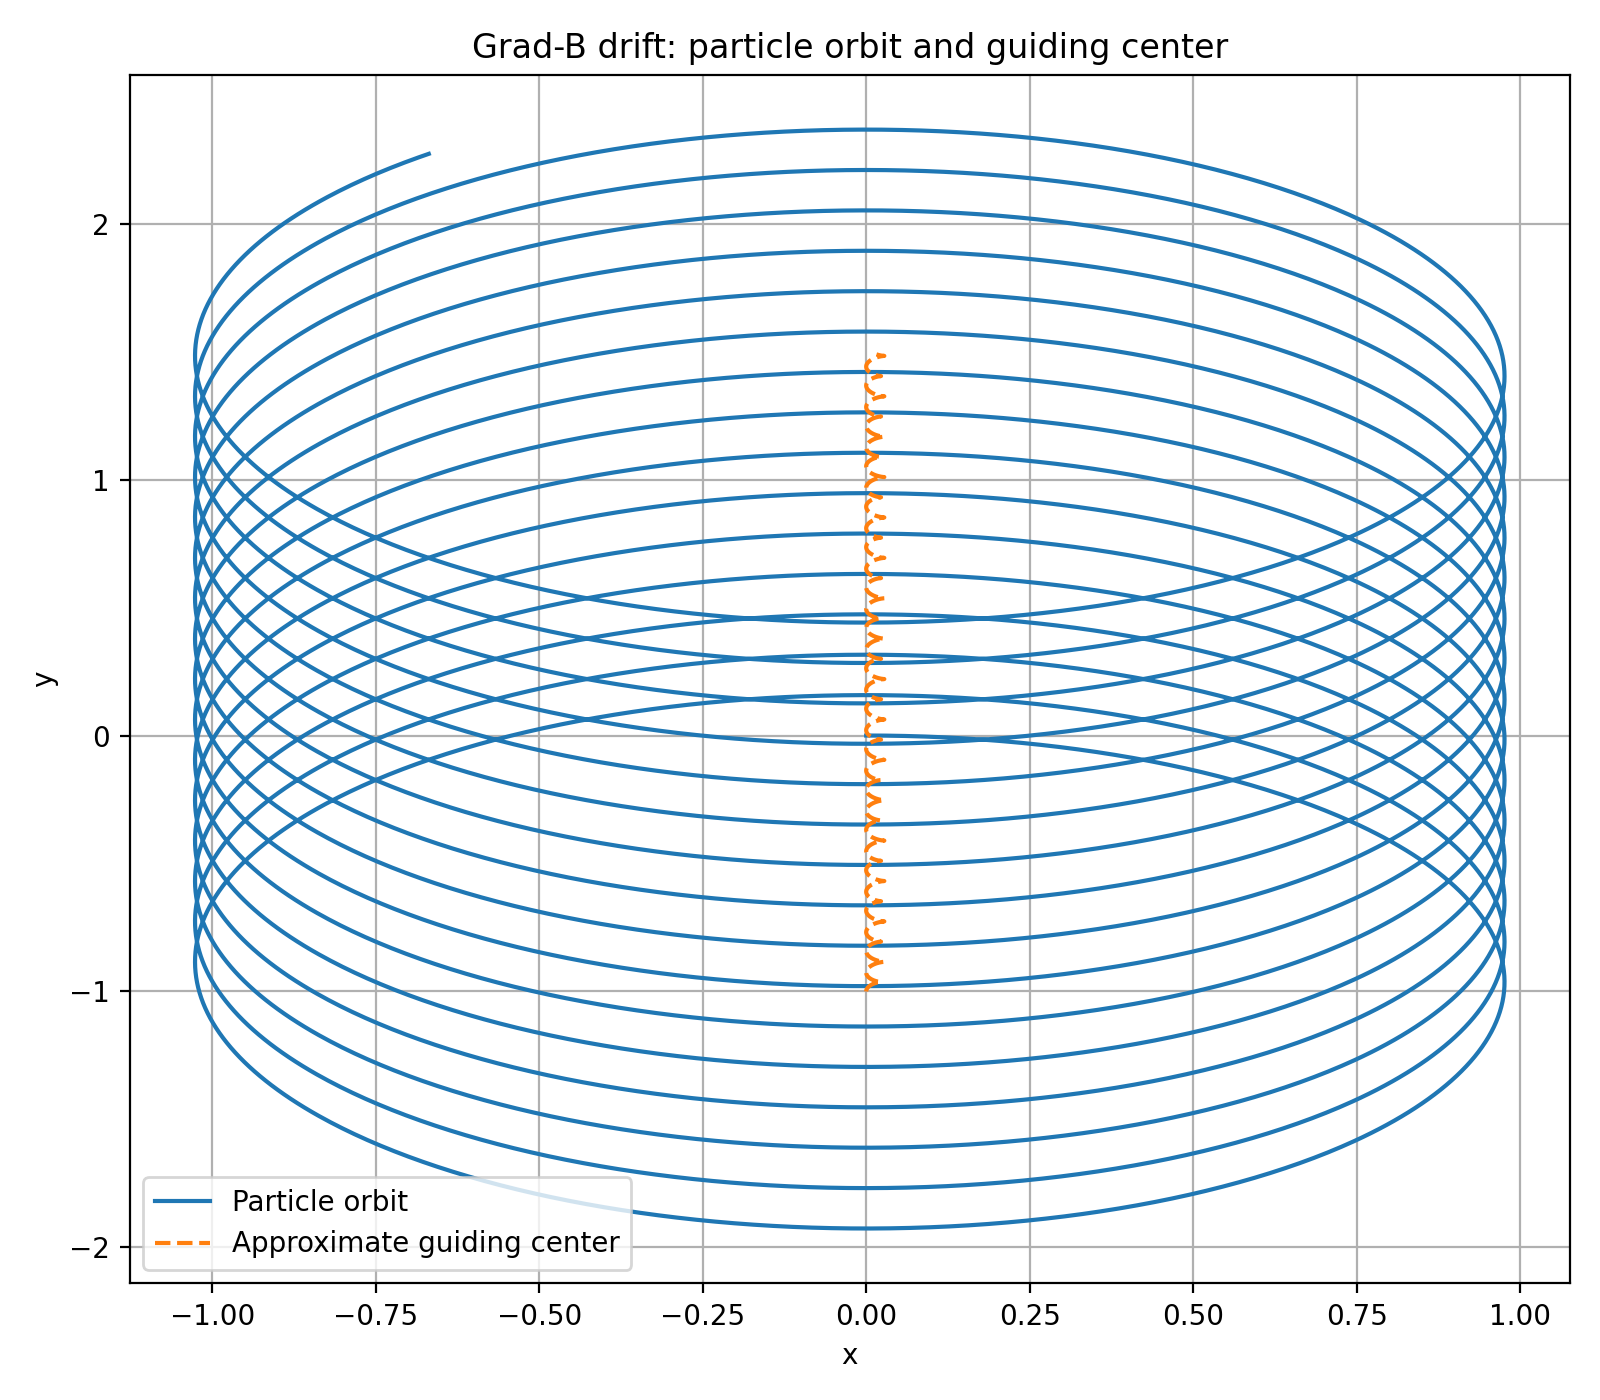
\includegraphics[width=\linewidth]{gradB_xy_orbit.png}
        \caption{Particle orbit and approximate guiding center.}
    \end{subfigure}\hfill
    \begin{subfigure}[t]{0.56\textwidth}
        \centering
        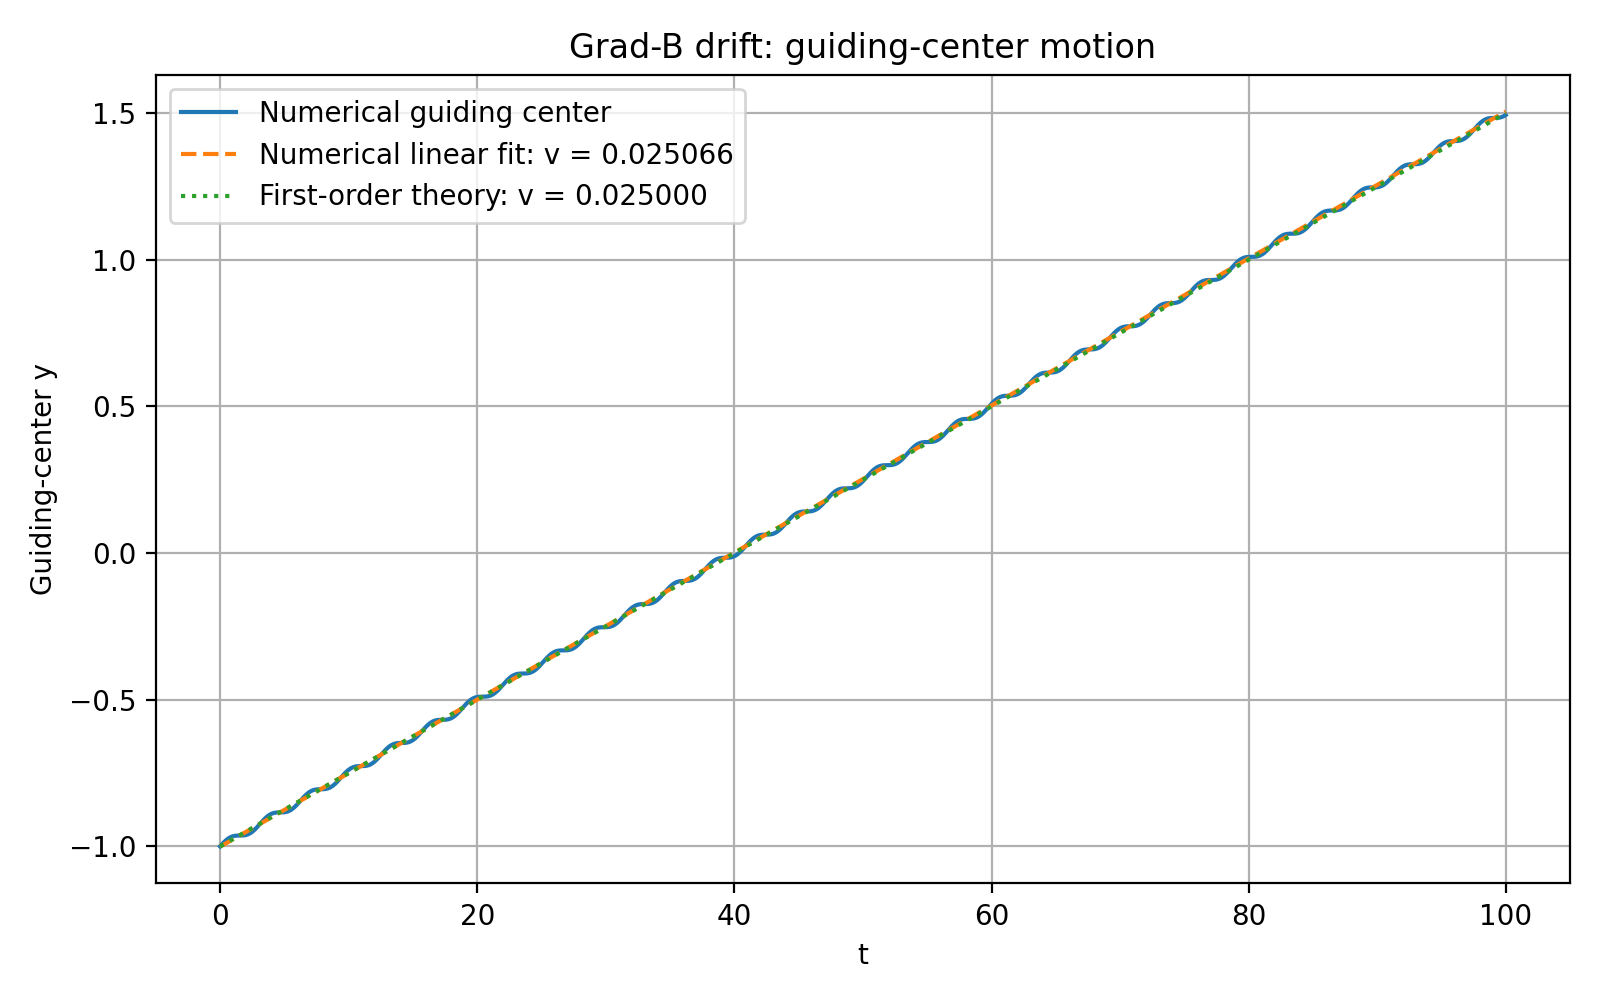
\includegraphics[width=\linewidth]{gradB_guiding_center.png}
        \caption{Numerical drift versus first-order theory.}
    \end{subfigure}
    \caption{Grad-$B$ drift for a weakly nonuniform magnetic field.}
    \label{fig:gradb}
\end{figure}

Because $\vect{E}=0$, the kinetic energy must remain constant. The maximum relative kinetic-energy error is $1.35\times10^{-10}$. The instantaneous diagnostic $\mu=m v_\perp^2/(2B)$ exhibits gyro-scale modulation with a maximum variation of about $5.4\%$; the relevant adiabatic statement concerns the slowly varying or gyro-averaged magnetic moment rather than the instantaneous value at every point of the finite-radius orbit.

\begin{figure}[H]
    \centering
    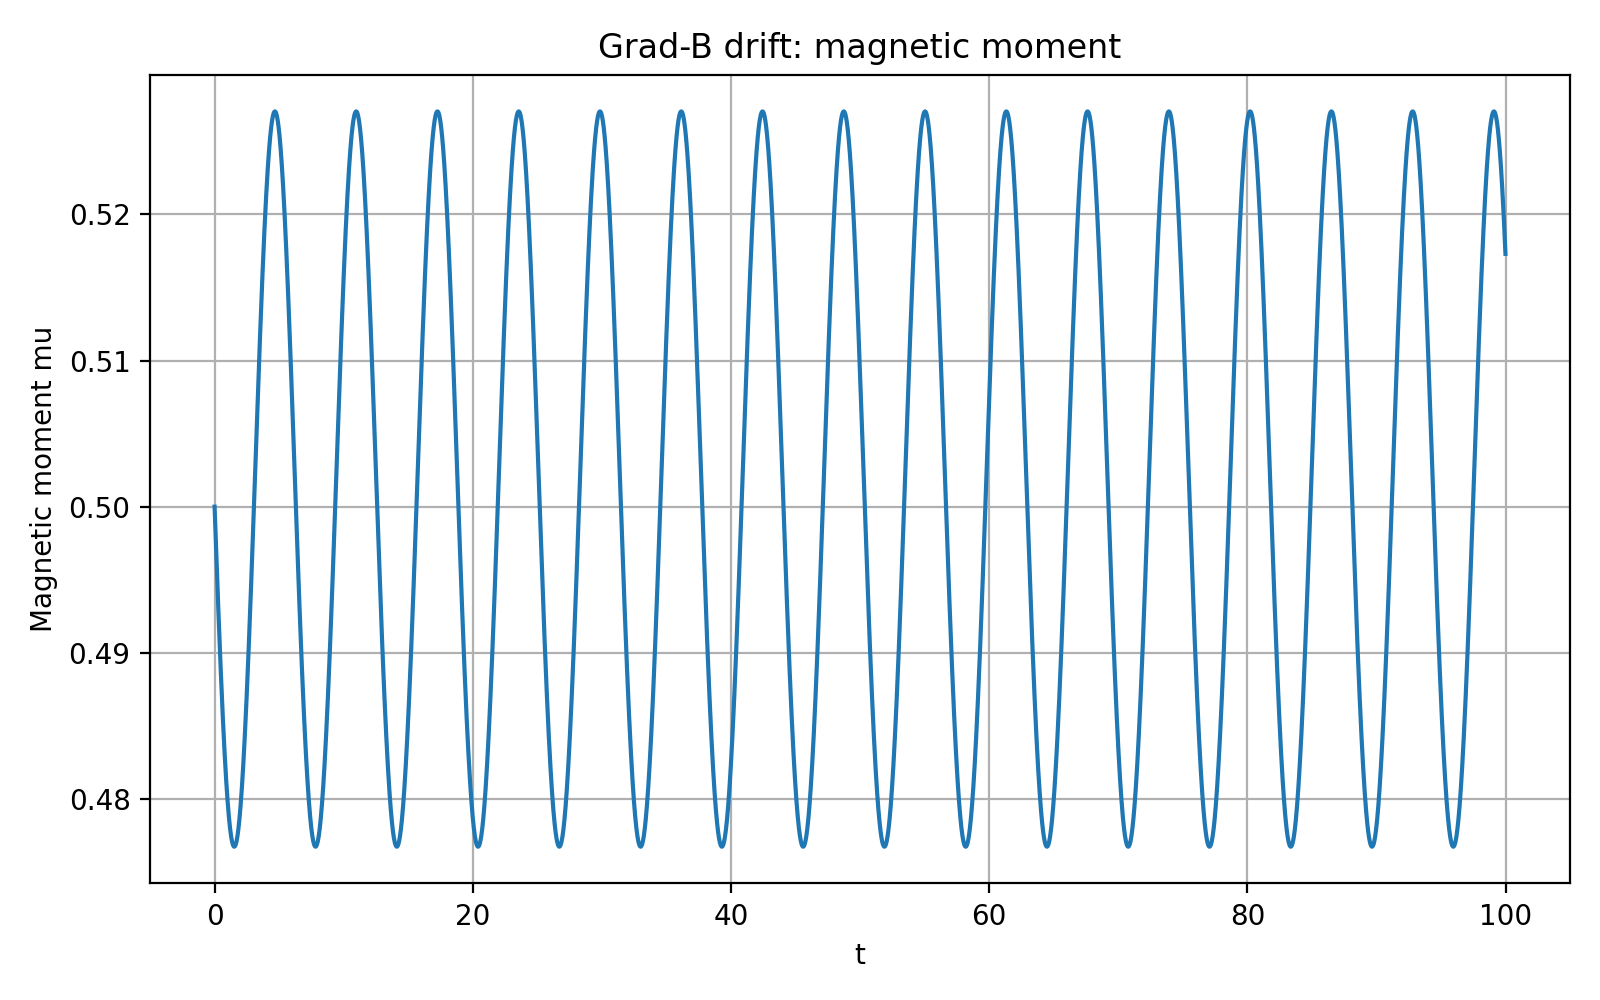
\includegraphics[width=0.68\textwidth]{gradB_magnetic_moment.png}
    \caption{Instantaneous magnetic moment in the grad-$B$ case. The oscillation occurs at the fast orbital scale while the secular drift remains slow.}
    \label{fig:gradb_mu}
\end{figure}

\subsection{Curvature drift}

To study curvature without simultaneously introducing $\nabla|B|$, a constant-magnitude azimuthal field is used:
\begin{equation}
    \vect{B}=B_0\hat{\vect{e}}_\phi
    =B_0\left(-\frac{y}{R},\frac{x}{R},0\right),
    \qquad R=\sqrt{x^2+y^2}.
    \label{eq:curvaturefield}
\end{equation}
The field lines are circles, $|\vect{B}|=B_0$, and $\nabla\cdot\vect{B}=0$ away from the cylindrical axis. For circular field lines,
\begin{equation}
    \vect{\kappa}=(\vect{b}\cdot\nabla)\vect{b}
    =-\frac{\hat{\vect{e}}_R}{R},
\end{equation}
and the first-order curvature drift is
\begin{equation}
    \boxed{
    \vc=\frac{m v_\parallel^2}{qB}\,\vect{b}\times\vect{\kappa}
    }.
    \label{eq:curvdrift}
\end{equation}
At $R_c=10$ with $v_\parallel=1$ and $v_\perp=0.2$, the theory predicts $v_{c,z}=0.100000$. The measured guiding-center velocity is $0.09727577$, corresponding to a $2.72\%$ difference. The guiding-center radius remains constant to approximately $5\times10^{-12}$ relative variation, and kinetic energy is conserved to approximately $6\times10^{-12}$.

\begin{figure}[H]
    \centering
    \begin{subfigure}[t]{0.44\textwidth}
        \centering
        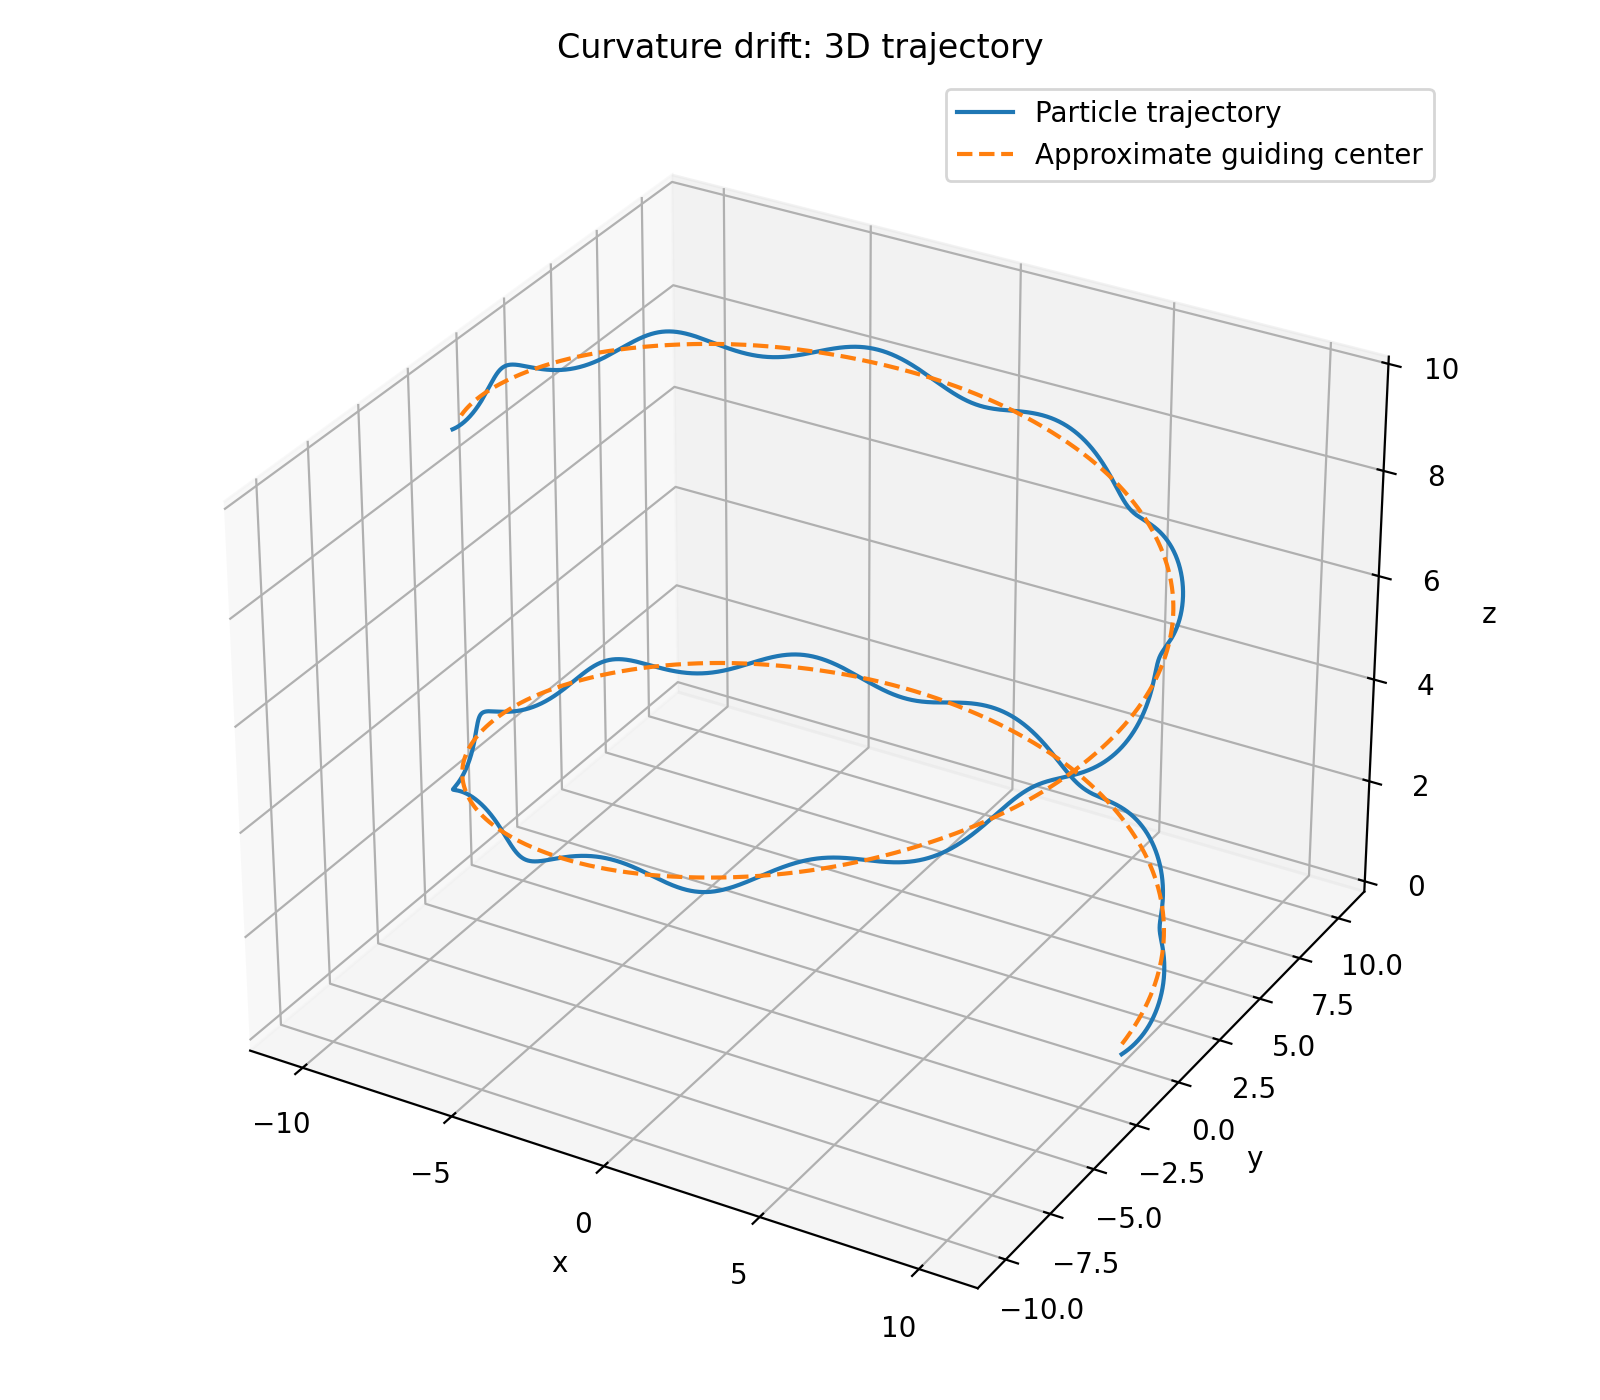
\includegraphics[width=\linewidth]{curvature_3d_trajectory.png}
        \caption{Particle and guiding-center trajectories.}
    \end{subfigure}\hfill
    \begin{subfigure}[t]{0.54\textwidth}
        \centering
        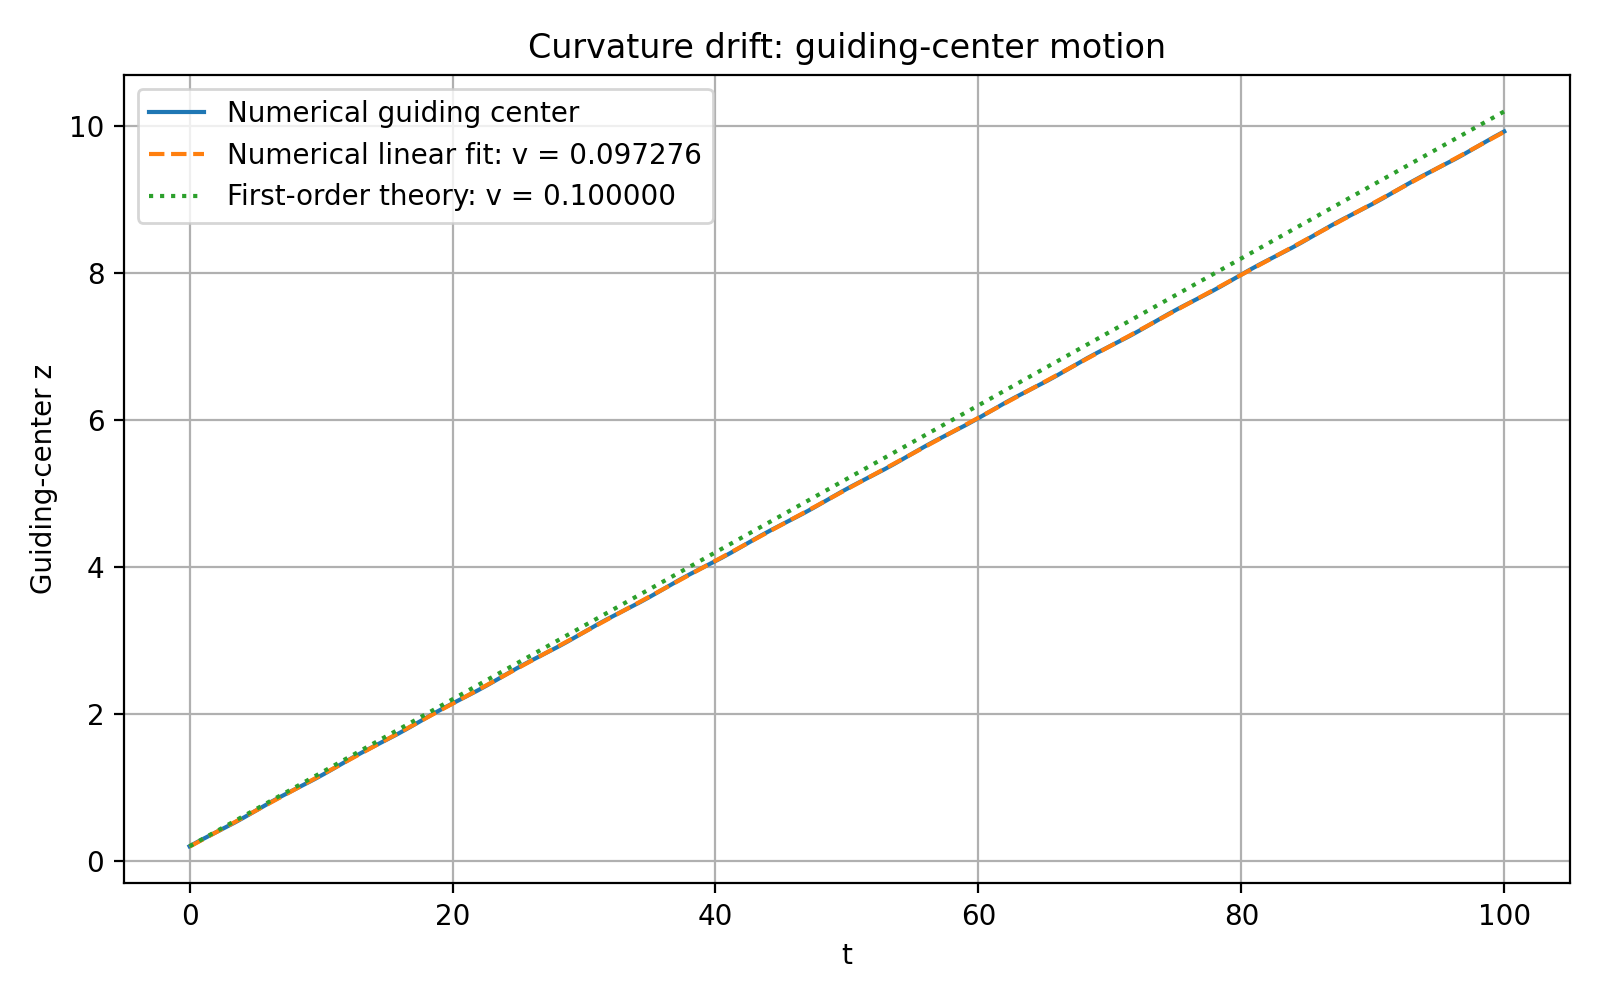
\includegraphics[width=\linewidth]{curvature_guiding_center.png}
        \caption{Drift in $z$: numerical result and theory.}
    \end{subfigure}
    \caption{Curvature drift generated by circular, constant-magnitude magnetic-field lines.}
    \label{fig:curvature}
\end{figure}

\subsection{Spatially nonuniform electric field and finite-Larmor-radius correction}

The nonuniform-electric-field benchmark uses
\begin{equation}
    \vect{E}(x)=E_0\cos(kx)\hat{\vect{x}},
    \qquad
    \vect{B}=B_0\hat{\vect{z}},
    \label{eq:nonuniformefield}
\end{equation}
with $E_0=0.02$ and $k=0.4$. This field is electrostatic, with potential
\begin{equation}
    \phi(x)=-\frac{E_0}{k}\sin(kx).
\end{equation}
The particle has $\rhL=1$, so $k\rhL=0.4$. Because the Larmor radius is finite, the particle samples different values of $E_x$ during one gyro-orbit. The local zero-Larmor-radius approximation therefore receives a finite-Larmor-radius (FLR) correction. For $k\rhL\ll1$,
\begin{equation}
    \left\langle\vE\right\rangle
    \simeq
    \left(1-\frac{k^2\rhL^2}{4}\right)
    \frac{\vect{E}(\vect{R}_{gc})\times\vect{B}}{B^2}.
    \label{eq:flrsecondorder}
\end{equation}
For a circular unperturbed gyro-orbit, the complete gyro-average is proportional to the Bessel factor $J_0(k\rhL)$; the analysis script evaluates the same average directly over gyro-angle without requiring an additional special-function library.

The local $E\times B$ estimate is $-0.020000$. The second-order FLR estimate is $-0.019200$, and the direct gyro-average gives $-0.01920796$. The full-orbit simulation gives
\begin{equation}
    v_{gc,y}^{\rm num}=-0.01920650.
\end{equation}
Thus the simulation differs from the local $E\times B$ approximation by $3.97\%$, but agrees with the direct gyro-average to $0.00764\%$. This clearly separates a physical FLR correction from numerical integration error.

\begin{figure}[H]
    \centering
    \begin{subfigure}[t]{0.44\textwidth}
        \centering
        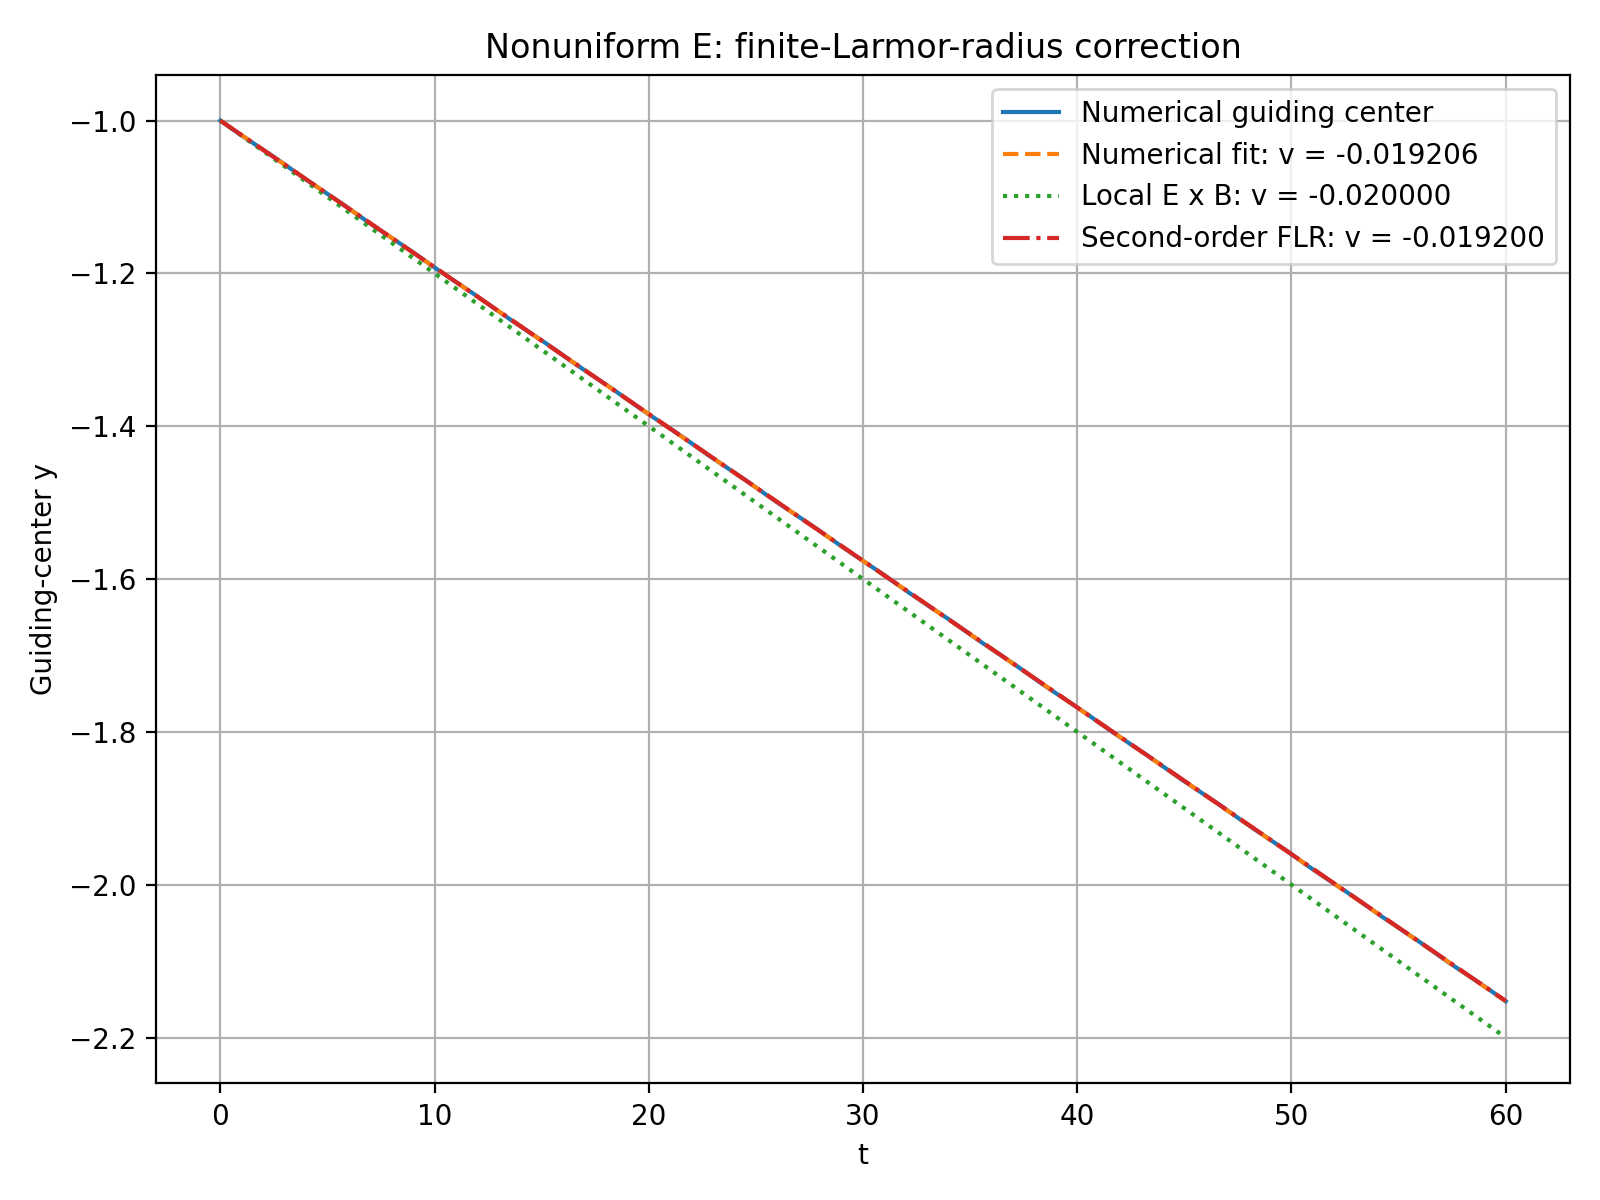
\includegraphics[width=\linewidth]{nonuniform_E_guiding_center.png}
        \caption{Full-orbit drift versus local and FLR predictions.}
    \end{subfigure}\hfill
    \begin{subfigure}[t]{0.54\textwidth}
        \centering
        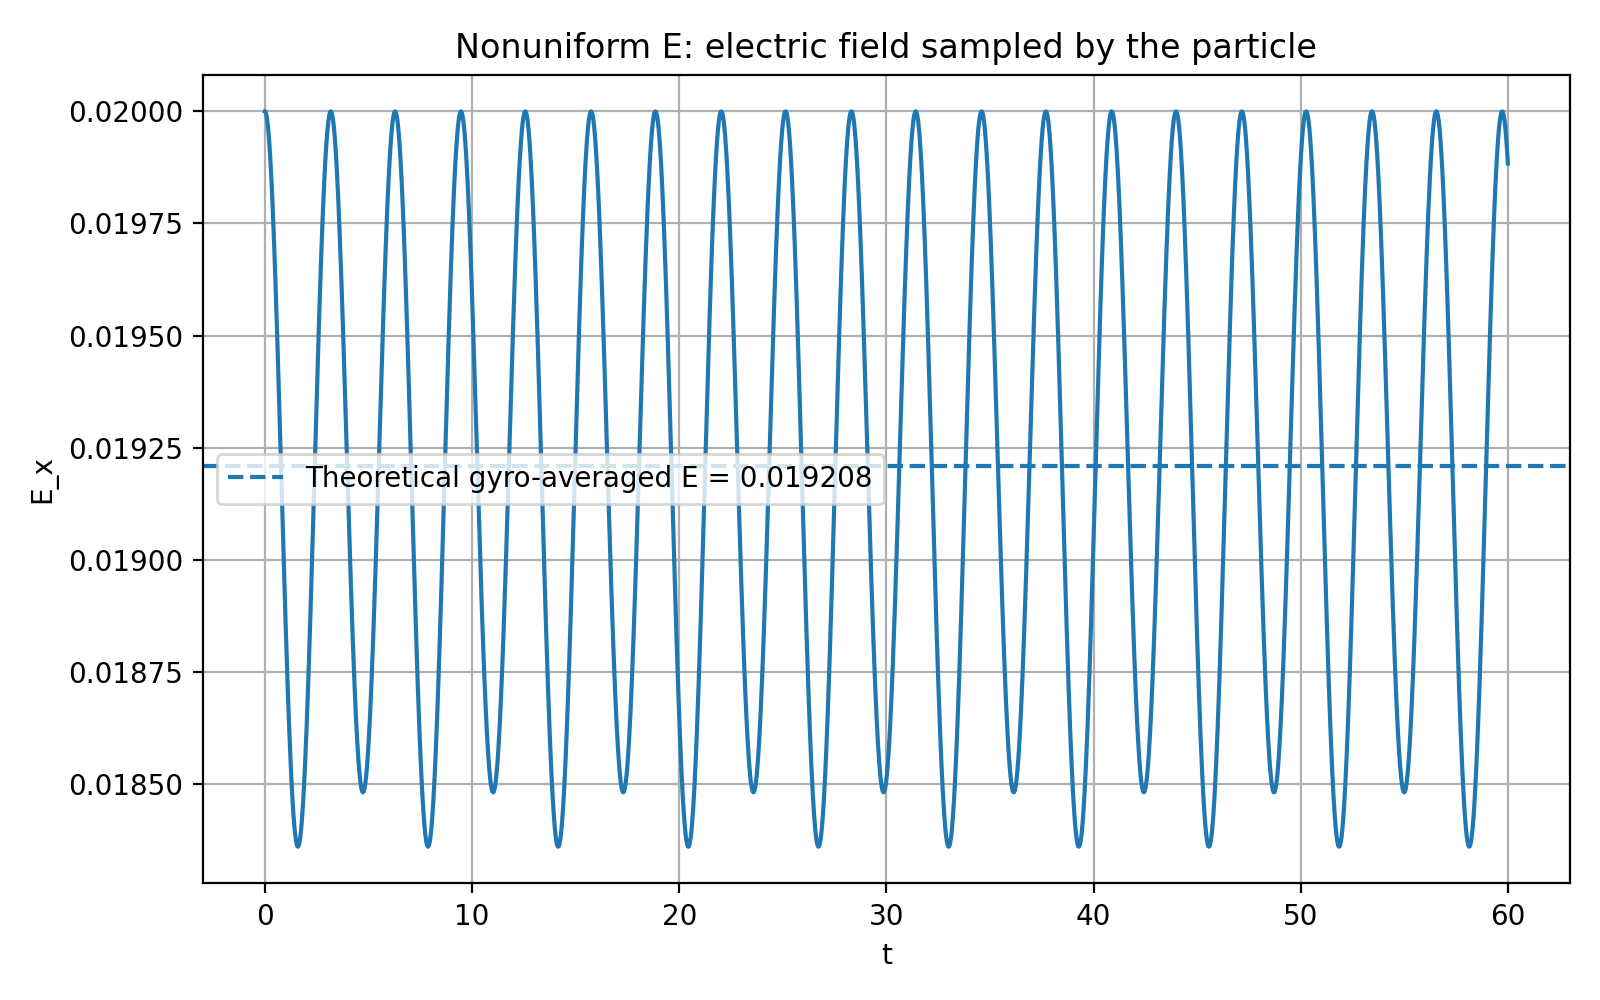
\includegraphics[width=\linewidth]{nonuniform_E_sampled_field.png}
        \caption{Electric field sampled around the gyro-orbit.}
    \end{subfigure}
    \caption{Finite-Larmor-radius effect in a spatially varying electrostatic field.}
    \label{fig:nonuniformE}
\end{figure}

The guiding-center $X$ coordinate remains constant to numerical precision. In addition, the conserved electrostatic total energy
\begin{equation}
    \mathcal{H}=K+q\phi
\end{equation}
has a maximum relative error of $8.11\times10^{-11}$.

\subsection{Polarization drift}

The final case uses a slowly varying perpendicular electric field,
\begin{equation}
    \vect{E}(t)=E_0\cos(\omega_E t)\hat{\vect{x}},
    \qquad
    \vect{B}=B_0\hat{\vect{z}},
    \label{eq:polarizationfield}
\end{equation}
with $E_0=0.2$ and $\omega_E=0.05$. Since $\Ohm=1$,
\begin{equation}
    \frac{\omega_E}{\Ohm}=0.05\ll1,
\end{equation}
which is the slowly varying regime used to derive polarization drift. To first order,
\begin{align}
    v_{E,y}(t) &= -\frac{E_0}{B_0}\cos(\omega_E t),\\
    \boxed{
    v_{p,x}(t)=\frac{m}{qB_0^2}\frac{dE_x}{dt}
    =-\frac{mE_0\omega_E}{qB_0^2}\sin(\omega_E t)
    }.
    \label{eq:polarization}
\end{align}
The corresponding first-order amplitudes are $|v_E|=0.2000$ and $|v_p|=0.0100$.

Because the forcing frequency is finite rather than zero, the exact slow response differs from first-order drift theory by
\begin{equation}
    \frac{1}{1-(\omega_E/\Ohm)^2}=1.00250627,
\end{equation}
giving slow-response amplitudes $0.20050125$ in $y$ and $0.01002506$ in $x$. For this benchmark, the forced full-orbit equations can also be solved exactly, providing a particularly strong independent test of the C++ trajectory. The maximum numerical-exact errors are approximately $3.2\times10^{-11}$ in position and $1.1\times10^{-11}$ in velocity.

\begin{figure}[H]
    \centering
    \begin{subfigure}[t]{0.49\textwidth}
        \centering
        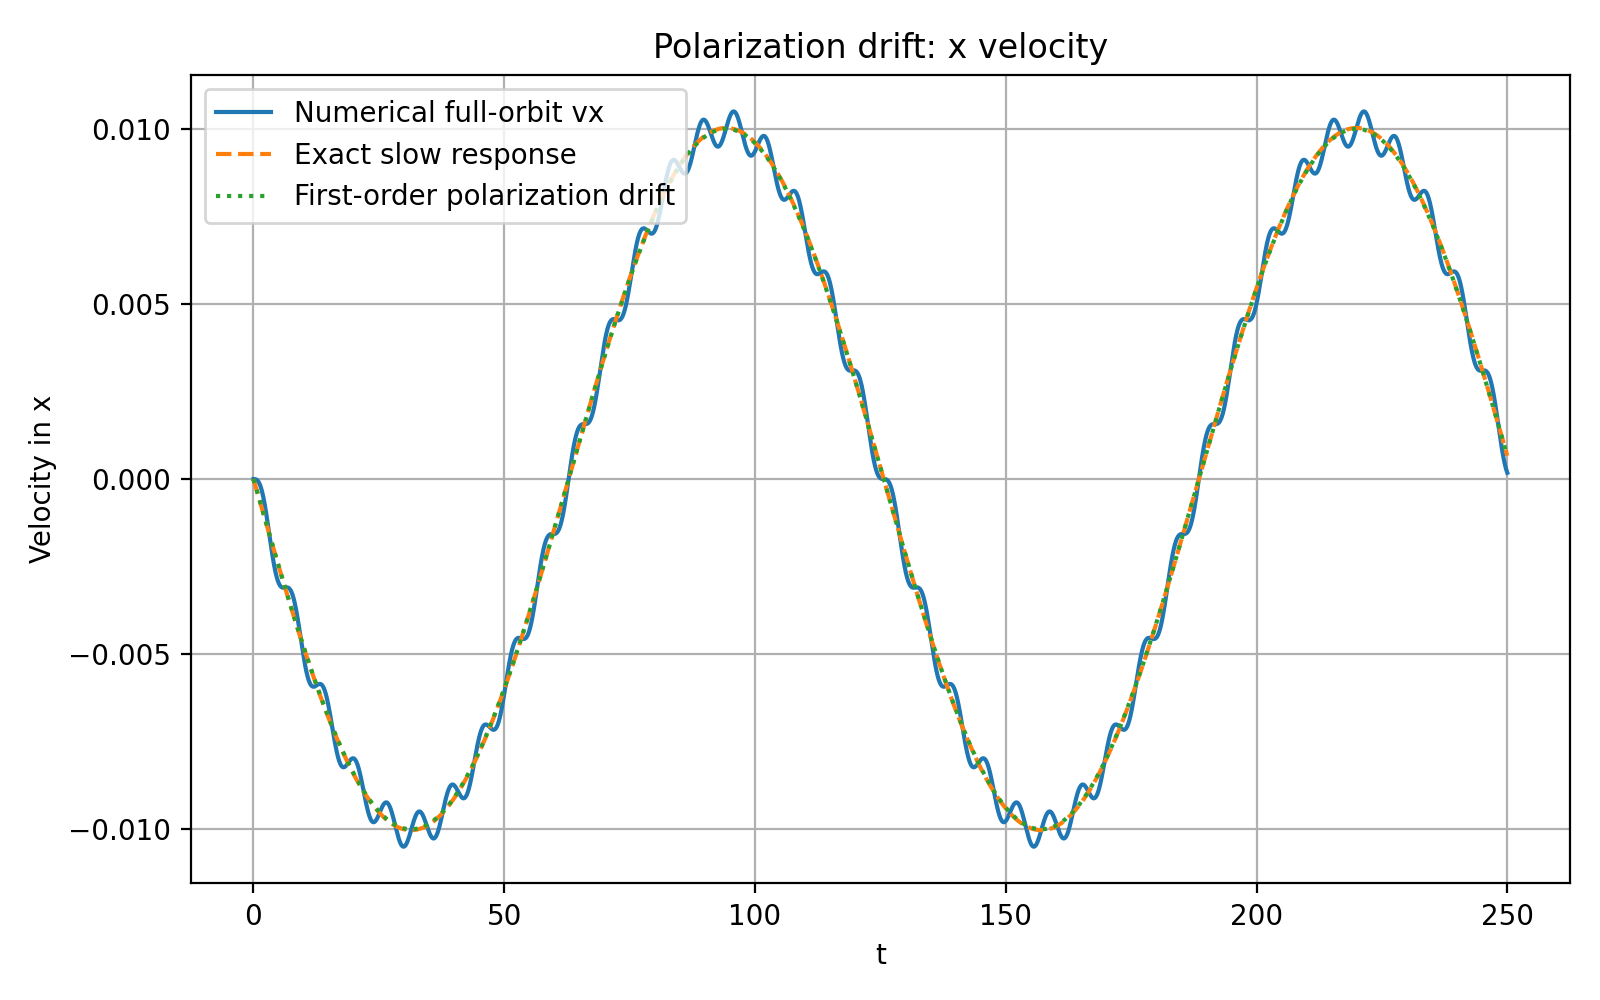
\includegraphics[width=\linewidth]{polarization_velocity_x.png}
        \caption{Polarization response in the $x$ velocity.}
    \end{subfigure}\hfill
    \begin{subfigure}[t]{0.49\textwidth}
        \centering
        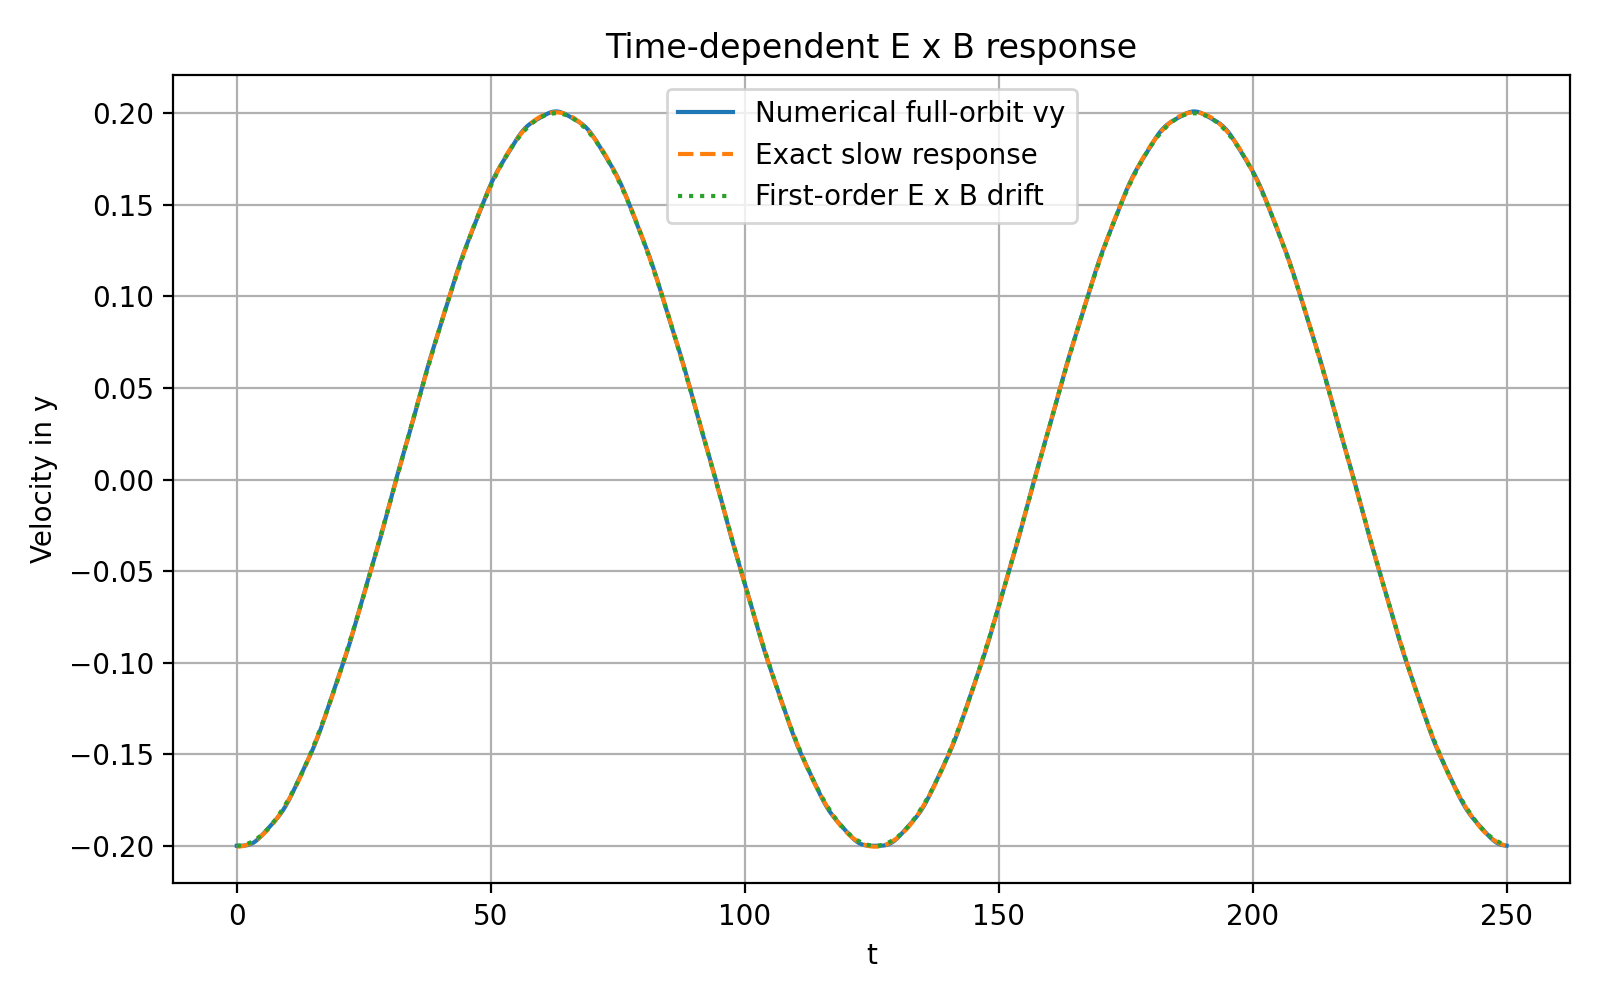
\includegraphics[width=\linewidth]{polarization_exb_velocity_y.png}
        \caption{Time-dependent $E\times B$ response in $y$.}
    \end{subfigure}
    \caption{Polarization benchmark. The full orbit follows the exact finite-frequency response, while the first-order drift theory gives the expected low-frequency limit.}
    \label{fig:polarization_velocity}
\end{figure}

\begin{figure}[H]
    \centering
    \begin{subfigure}[t]{0.41\textwidth}
        \centering
        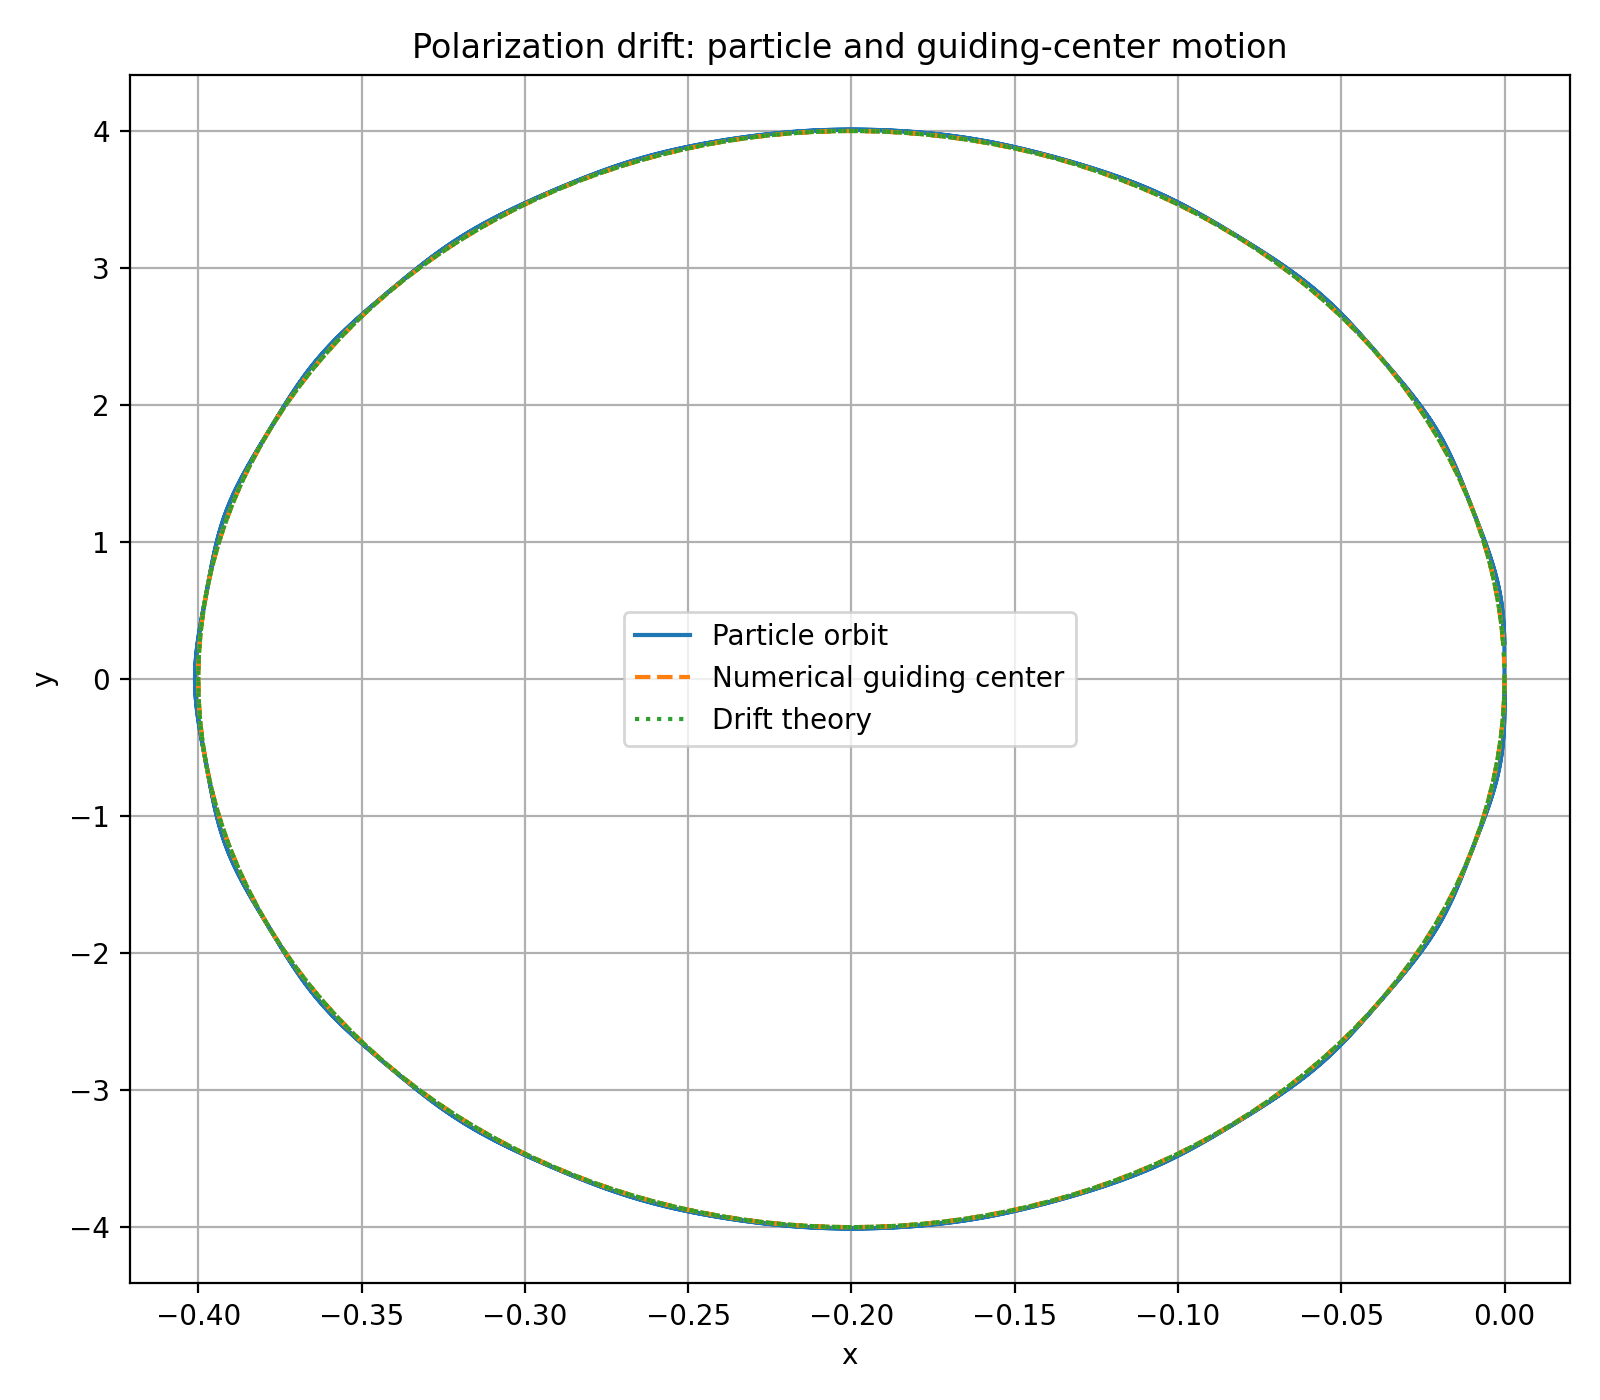
\includegraphics[width=\linewidth]{polarization_xy_motion.png}
        \caption{Perpendicular orbit: numerical and exact solution.}
    \end{subfigure}\hfill
    \begin{subfigure}[t]{0.57\textwidth}
        \centering
        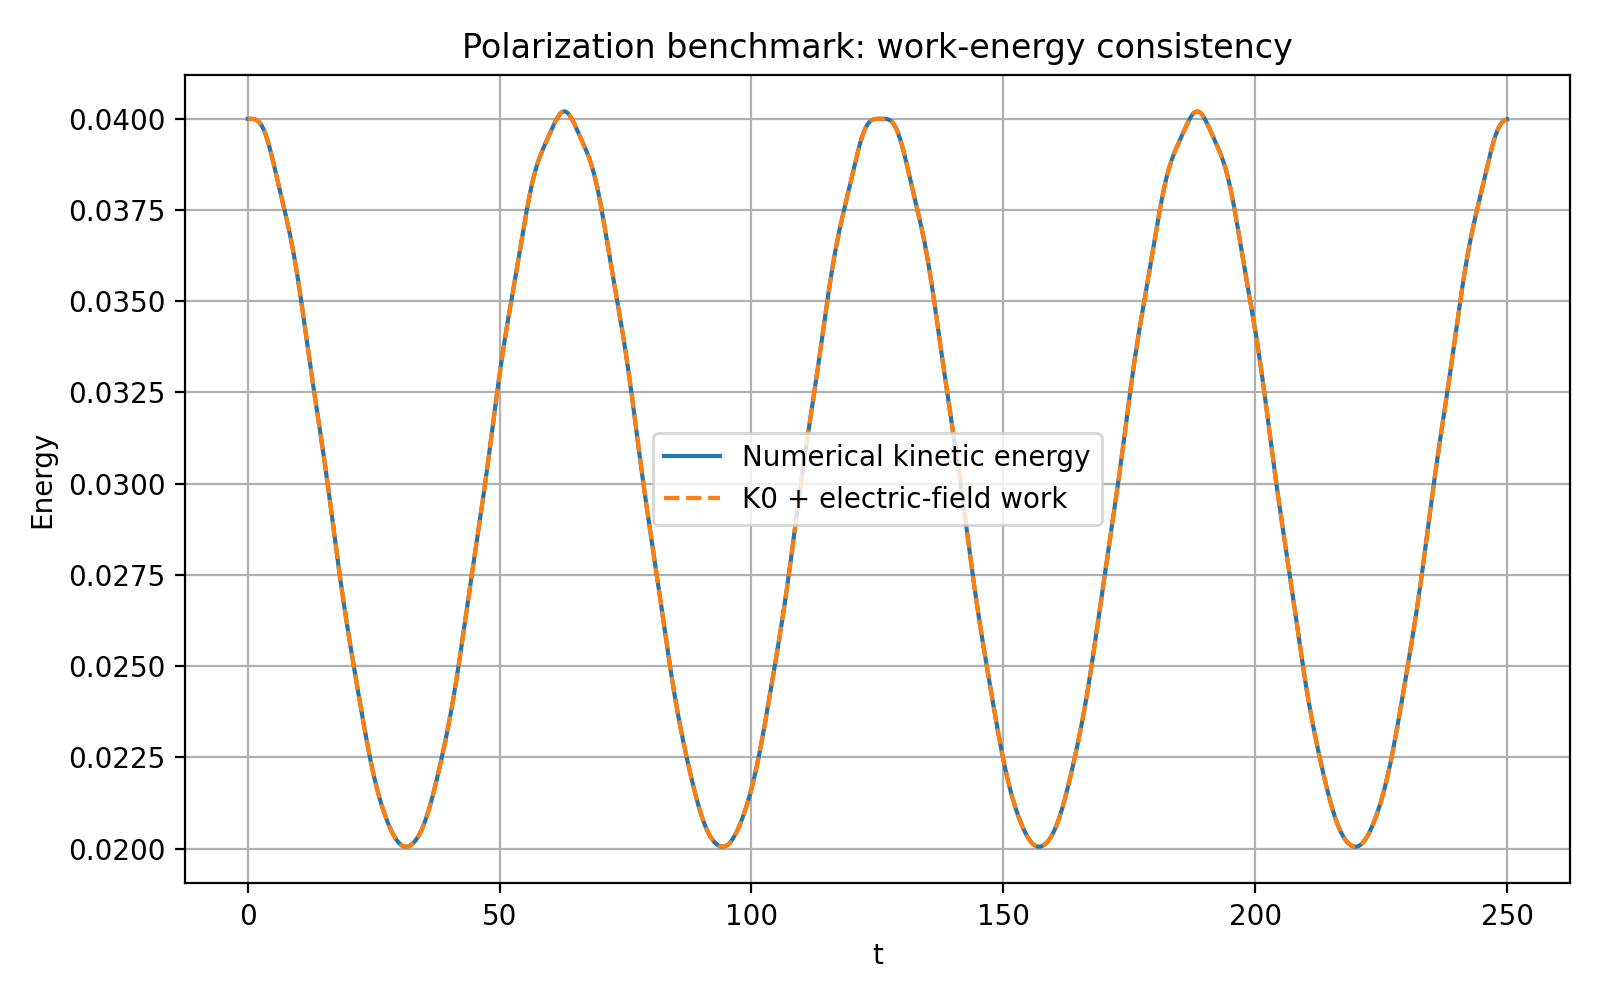
\includegraphics[width=\linewidth]{polarization_energy.png}
        \caption{Kinetic energy and electric-field work.}
    \end{subfigure}
    \caption{Independent checks for the polarization case. The work-energy relation $K(t)-K(0)=\int q\vect{E}\cdot\vect{v}\,dt$ is satisfied to approximately $1.7\times10^{-9}$ in absolute energy.}
    \label{fig:polarization_checks}
\end{figure}

% --------------------------------------------------
\section{Quantitative Summary}
% --------------------------------------------------

\begin{table}[H]
    \centering
    \small
    \caption{Comparison of numerical results with the relevant theoretical prediction.}
    \resizebox{\textwidth}{!}{%
    \begin{tabular}{lllll}
        \toprule
        \textbf{Case} & \textbf{Reference prediction} & \textbf{Theory} & \textbf{Numerical} & \textbf{Difference} \\
        \midrule
        $E\times B$ & $v_{E,y}$ & $-0.10000000$ & $-0.10000000$ & $1.1\times10^{-13}$ relative \\
        Grad-$B$ & $v_{\nabla B,y}$ & $0.02500000$ & $0.02506606$ & $0.264\%$ \\
        Curvature & $v_{c,z}$ & $0.10000000$ & $0.09727577$ & $2.72\%$ \\
        Nonuniform $E$ & gyro-averaged $v_y$ & $-0.01920796$ & $-0.01920650$ & $0.00764\%$ \\
        Polarization & exact full orbit & analytical trajectory & numerical trajectory & $\sim10^{-11}$ orbit error \\
        \bottomrule
    \end{tabular}}
    \label{tab:summary}
\end{table}

The exact-solvable benchmarks ($B$ uniform, crossed uniform fields, and the forced polarization case) test the numerical integrator itself. The grad-$B$ and curvature cases instead test the agreement between the full orbit and reduced first-order guiding-center theory, so their percent-level discrepancies should not be interpreted as RK4 errors. The nonuniform-$E$ benchmark demonstrates this distinction particularly clearly: the numerical result strongly disagrees with the zero-Larmor-radius approximation but agrees with the finite-Larmor-radius gyro-average.

% --------------------------------------------------
\section{Discussion}
% --------------------------------------------------

The simulations show the scale separation that motivates guiding-center theory: a rapid cyclotron orbit is superimposed on a much slower cross-field displacement. However, the physical origin of the slow motion differs between the cases.

\begin{itemize}
    \item The $\vect{E}\times\vect{B}$ drift is an exact common drift for both charge signs and does not depend on $m$ or $q$.
    \item Grad-$B$ and curvature drifts depend on particle properties and arise from magnetic-field nonuniformity or field-line geometry. Their formulas are asymptotic guiding-center results rather than exact full-orbit solutions.
    \item A spatially nonuniform electric field illustrates finite-Larmor-radius physics: the particle samples the field over its whole gyro-orbit, so evaluating $\vect{E}$ only at the guiding center is insufficient when $k\rhL$ is finite.
    \item Polarization drift is a temporal inertial correction. It is smaller than the time-dependent $E\times B$ motion by a factor of order $\omega_E/\Ohm$ in the low-frequency limit.
\end{itemize}

The field models were chosen to isolate each effect as cleanly as possible. In particular, the grad-$B$ field satisfies $\nabla\cdot\vect{B}=0$, while the curvature benchmark keeps $|B|$ constant so that curvature drift is not mixed with grad-$B$ drift. The nonuniform electric field is electrostatic, allowing conservation of $K+q\phi$ to be checked independently.

% --------------------------------------------------
\section{Conclusions}
% --------------------------------------------------

A compact three-dimensional full-orbit simulator was implemented in C++17 using the Lorentz equation and a fourth-order Runge-Kutta method. The same integrator was used for all required cases, while only the prescribed electromagnetic field and initial conditions were changed. Independent Python scripts were used for analytical validation, guiding-center reconstruction, conservation diagnostics, fitting, and visualization.

All five requested drift phenomena were reproduced:
\begin{itemize}
    \item uniform crossed fields produced the expected $\vect{E}\times\vect{B}$ drift;
    \item a weak magnetic gradient produced the expected grad-$B$ drift;
    \item circular constant-magnitude field lines produced curvature drift;
    \item a spatially varying electrostatic field showed the expected finite-Larmor-radius correction; and
    \item a slowly time-varying electric field produced polarization drift together with the time-dependent $\vect{E}\times\vect{B}$ response.
\end{itemize}

The exact-solvable cases agree with analytical full-orbit solutions at approximately $10^{-9}$--$10^{-11}$, demonstrating that the numerical errors are much smaller than the physical guiding-center approximation errors in the nonuniform cases. The project therefore provides a direct numerical demonstration of how the familiar drift velocities emerge from the complete Lorentz dynamics rather than being imposed as separate equations of motion.

% --------------------------------------------------
\begin{thebibliography}{9}

\bibitem{Chen2016}
F. F. Chen,
\textit{Introduction to Plasma Physics and Controlled Fusion},
3rd ed., Springer, 2016.

\end{thebibliography}

\end{document}
